% Options for packages loaded elsewhere
\PassOptionsToPackage{unicode}{hyperref}
\PassOptionsToPackage{hyphens}{url}
%
\documentclass[
]{book}
\usepackage{lmodern}
\usepackage{amssymb,amsmath}
\usepackage{ifxetex,ifluatex}
\ifnum 0\ifxetex 1\fi\ifluatex 1\fi=0 % if pdftex
  \usepackage[T1]{fontenc}
  \usepackage[utf8]{inputenc}
  \usepackage{textcomp} % provide euro and other symbols
\else % if luatex or xetex
  \usepackage{unicode-math}
  \defaultfontfeatures{Scale=MatchLowercase}
  \defaultfontfeatures[\rmfamily]{Ligatures=TeX,Scale=1}
\fi
% Use upquote if available, for straight quotes in verbatim environments
\IfFileExists{upquote.sty}{\usepackage{upquote}}{}
\IfFileExists{microtype.sty}{% use microtype if available
  \usepackage[]{microtype}
  \UseMicrotypeSet[protrusion]{basicmath} % disable protrusion for tt fonts
}{}
\makeatletter
\@ifundefined{KOMAClassName}{% if non-KOMA class
  \IfFileExists{parskip.sty}{%
    \usepackage{parskip}
  }{% else
    \setlength{\parindent}{0pt}
    \setlength{\parskip}{6pt plus 2pt minus 1pt}}
}{% if KOMA class
  \KOMAoptions{parskip=half}}
\makeatother
\usepackage{xcolor}
\IfFileExists{xurl.sty}{\usepackage{xurl}}{} % add URL line breaks if available
\IfFileExists{bookmark.sty}{\usepackage{bookmark}}{\usepackage{hyperref}}
\hypersetup{
  pdftitle={Quantitative Research Methods \& Analysis: Exercises},
  pdfauthor={Matthew J. C. Crump, Anjali Krishnan, Stephen Volz, and Alla Chavarga; Adapted for use at EUC by Thomas Hulst},
  hidelinks,
  pdfcreator={LaTeX via pandoc}}
\urlstyle{same} % disable monospaced font for URLs
\usepackage{longtable,booktabs}
% Correct order of tables after \paragraph or \subparagraph
\usepackage{etoolbox}
\makeatletter
\patchcmd\longtable{\par}{\if@noskipsec\mbox{}\fi\par}{}{}
\makeatother
% Allow footnotes in longtable head/foot
\IfFileExists{footnotehyper.sty}{\usepackage{footnotehyper}}{\usepackage{footnote}}
\makesavenoteenv{longtable}
\usepackage{graphicx,grffile}
\makeatletter
\def\maxwidth{\ifdim\Gin@nat@width>\linewidth\linewidth\else\Gin@nat@width\fi}
\def\maxheight{\ifdim\Gin@nat@height>\textheight\textheight\else\Gin@nat@height\fi}
\makeatother
% Scale images if necessary, so that they will not overflow the page
% margins by default, and it is still possible to overwrite the defaults
% using explicit options in \includegraphics[width, height, ...]{}
\setkeys{Gin}{width=\maxwidth,height=\maxheight,keepaspectratio}
% Set default figure placement to htbp
\makeatletter
\def\fps@figure{htbp}
\makeatother
\setlength{\emergencystretch}{3em} % prevent overfull lines
\providecommand{\tightlist}{%
  \setlength{\itemsep}{0pt}\setlength{\parskip}{0pt}}
\setcounter{secnumdepth}{5}
\usepackage{booktabs}
\usepackage{amsthm}
\usepackage{amsmath}
\usepackage{marginnote}
\makeatletter
\def\thm@space@setup{%
  \thm@preskip=8pt plus 2pt minus 4pt
  \thm@postskip=\thm@preskip
}
\makeatother
\usepackage[]{natbib}
\bibliographystyle{apalike}

\title{Quantitative Research Methods \& Analysis: Exercises}
\author{Matthew J. C. Crump, Anjali Krishnan, Stephen Volz, and Alla Chavarga \and Adapted for use at EUC by Thomas Hulst}
\date{Last Compiled 2020-11-25}

\begin{document}
\maketitle

{
\setcounter{tocdepth}{1}
\tableofcontents
}
\hypertarget{preface}{%
\chapter*{Preface}\label{preface}}
\addcontentsline{toc}{chapter}{Preface}

\hypertarget{important-notes}{%
\section{Important notes}\label{important-notes}}

This is the exercise manual for Quantitative Research Methods \& Analysis at EUC. As with the textbook, this manual was adapted from ``Answering questions with data'' by Mattew J.C. Crump.

The original text is part of a \href{https://osf.io/3s68c/}{larger OER (Open Educational Resource) course} for teaching undergraduate statistics in psychology. As such, the text assumes you are a psychology student and many of the examples are drawn from the field of psychology. This does not mean that this course is only useful for you if you have an interest in psychology. The field of psychology will serve as a vehicle to teach you important concepts and skills in quantitative research methods and data analysis, but the concepts and skills taught are universal.

This manual provides the exercises we will work on during tutorials. We use open-data sets that are usually paired with a primary research article. The manual is a free and open resource. See below for more information about copying, making change, or contributing to the lab manual.

\hypertarget{attributions}{%
\subsection{Attributions}\label{attributions}}

This lab manual was authored by Matt Crump. The exercises for weeks 6, 7, and 8 were adapted and expanded from \href{https://sites.trinity.edu/osl}{Open Stats Labs}. Thanks to Open Stats Labs (Dr.~Kevin P. McIntyre) for their fantastic work.

\hypertarget{cc-by-sa-4.0-license}{%
\subsection{CC BY-SA 4.0 license}\label{cc-by-sa-4.0-license}}

All resources are released under a creative commons licence \href{https://creativecommons.org/licenses/by-sa/4.0/}{CC BY-SA 4.0}. Click the link to read more about the license, or read more below:

This license means that you are free to:

\begin{itemize}
\tightlist
\item
  Share: copy and redistribute the material in any medium or format
\item
  Adapt: remix, transform, and build upon the material for any purpose, even commercially.
\end{itemize}

The licensor cannot revoke these freedoms as long as you follow the license terms.

Under the following terms:

\begin{itemize}
\tightlist
\item
  Attribution: You must give appropriate credit, provide a link to the license, and indicate if changes were made. You may do so in any reasonable manner, but not in any way that suggests the licensor endorses you or your use.
\item
  ShareAlike: If you remix, transform, or build upon the material, you must distribute your contributions under the same license as the original.
\item
  No additional restrictions: You may not apply legal terms or technological measures that legally restrict others from doing anything the license permits.
\end{itemize}

\hypertarget{week-1-introduction}{%
\chapter{Week 1: Introduction}\label{week-1-introduction}}

In this course we will be using R as a tool to analyze data, and as a tool to help us gain a better understanding of what our analyses are doing. Throughout each lab we will show you how to use R to solve specific problems, and then you will use the examples to solve homework and lab assignments. R is a very deep programming language, and in many ways we will only be skimming the surface of what R can do. Along the way, there will be many pointers to more advanced techniques that interested students can follow to become experts in using R for data-analysis, and computer programming in general.

R is primarily a computer programming language for statistical analysis. It is \emph{free}, and \emph{open-source} (many people contribute to developing it), and runs on most operating systems. It is a powerful language that can be used for all sorts of mathematical operations, data-processing, analysis, and graphical display of data. I even used R to write this lab manual. And, I use R all the time for my own research, because it makes data-analyis fast, efficient, transparent, reproducible, and exciting.

Statistics Software

\begin{itemize}
\tightlist
\item
  \href{http://www-01.ibm.com/software/analytics/spss/}{SPSS}
\item
  \href{http://www.sas.com/en_us/home.html}{SAS}
\item
  \href{http://www.jmp.com}{JMP}
\item
  \href{http://www.r-project.org}{R}
\item
  \href{http://julialang.org}{Julia}
\item
  \href{http://www.mathworks.com/products/matlab/}{Matlab}
\end{itemize}

\hypertarget{why-r}{%
\subsection{Why R?}\label{why-r}}

There are lots of different options for using computers to analyze data, why use R?. The options all have pros and cons, and can be used in different ways to solve a range of different problems. Some software allows you to load in data, and then analyze the data by clicking different options in a menu. This can sometimes be fast and convenient. For example, once the data is loaded, all you have to do is click a couple buttons to analyse the data! However, many aspects of data-analysis are not so easy. For example, particular analyses often require that the data be formatted in a particular way so that the program can analyze it properly. Often times when a researcher wants to ask a new question of an existing data set, they have to spend time re-formatting the data. If the data is large, then reformatting by hand is very slow, and can lead to errors. Another option, is to use a scripting language to instruct the computer how reformat the data. This is very fast and efficient. R provides the ability to everything all in one place. You can load in data, reformat it any way you like, then anlayze it anyway you like, and create beautiful graphs and tables (publication quality) to display your findings. Once you get the hang of R, it becomes very fast and efficient.

\hypertarget{installing-r-and-r-studio}{%
\subsection{Installing R and R Studio}\label{installing-r-and-r-studio}}

Download and install R onto your computer. The R website is: \url{http://www.r-project.org}

Find the download R using the link. This will take you to a page with many different mirror links. You can click any of these links to download a version of R that will work on your computer. After you have installed R you can continue.

After you have installed R on your computer, you should want to install another program called R studio. This program provides a user-friendly interface for using R. You must already have installed R before you perform this step. The R-studio website is: \url{http://www.rstudio.com}

Find the download link on the front-page, and then download R studio desktop version for your computer. After you have installed R studio you will be ready to start using R.

The website \href{http://www.r-fiddle.org}{R-fiddle} allows you to run R scripts in the cloud, so you can practice R from your web-browser!

\hypertarget{r-studio-notes-and-tips}{%
\subsection{R studio notes and tips}\label{r-studio-notes-and-tips}}

\begin{figure}
\centering
\includegraphics{figures/FigRstudio.pdf}
\caption{\label{fig:2rstudiod}The R-studio workspace}
\end{figure}

\hypertarget{console}{%
\subsubsection{Console}\label{console}}

When you open up R studio you will see three or four main windows (the placement of each are configurable). In the above example, the bottom left window is the command line (terminal or console) for R. This is used to directly enter commands into R. Once you have entered a command here, press enter to execute the command. The console is useful for entering single lines of code and running them. Oftentimes this occurs when you are learning how to correctly execute a line of code in R. Your first few attempts may be incorrect resulting in errors, but trying out different variations on your code in the command line can help you produce the correct code. Pressing the up arrow while in the console will scroll through the most recently executed lines of code.

\hypertarget{script-editor}{%
\subsubsection{Script Editor}\label{script-editor}}

The top left corner contains the script editor. This is a simple text editor for writing and saving R scripts with many lines. Several tabs can be opened at once, with each tab representing a different R script. R scripts can be saved from the editor (resulting in a .r file). Whole scripts can be run by copy and pasting them into the console and pressing enter. Alternatively, you can highlight portions of the script that you want to run (in the script editor) and press command-enter to automatically run that portion in the console (or press the button for running the current line/section: green arrow pointing right).

\hypertarget{workspace-and-history}{%
\subsubsection{Workspace and History}\label{workspace-and-history}}

The top right panel contains two tabs, one for the workspace and another for history. The workspace lists out all of the variables and functions that are currently loaded in R's memory. You can inspect each of the variables by clicking on them. This is generally only useful for variables that do not contain large amounts of information. The history tab provides a record of the recent commands executed in the console.

\hypertarget{file-plot-packages-help}{%
\subsubsection{File, Plot, Packages, Help}\label{file-plot-packages-help}}

The bottom-right window has four tabs for files, plots, packages, and help. The files tab allows browsing of the computers file directory. An important concept in R is the \textbf{current working directory}. This is file folder that R points to by default. Many functions in R will save things directly to this direct, or attempt to read files from this directory. The current working directory can be changed by navigating to the desired folder in the file menu, and then clicking on the more option to set that folder to the current working directory. This is especially important when reading in data to R. The current working directory should be set to the folder containing the data to be inputted into R. The plots tab will show recent plots and figures made in R. The packages tab lists the current R libraries loaded into memory, and provides the ability to download and enable new R packages. The help menu is an invaluable tool. Here, you can search for individual R commands to see examples of how they are used. Sometimes the help files for individual commands are opaque and difficult to understand, so it is necessary to do a Google search to find better examples of using these commands.

\hypertarget{how-to-complete-the-r-labs}{%
\subsection{How to complete the R Labs}\label{how-to-complete-the-r-labs}}

Each of the labs focuses on particular data-analysis problems, from graphing data, computing descriptive statistics, to running inferential tests in R. All of the labs come in three parts, a training part, a generalization part, and a writing part. The training part includes step-by-step examples of R code that solves particular problems. The R code is always highlighted in grey. The generalization part gives short assignments to change parts of the provided code to solve a new problem. The writing part tasks you with answering questions about statitiscal concepts.

The way to complete each lab is to open a new R Markdown document in R-studio, and then document your progression through each of the parts. By doing this, you will become familiar with how R and R-studio works, and how to create documents that preserve both the code and your notes all in one place. There are a few tricks to getting started that are outline below.

\begin{enumerate}
\def\labelenumi{\arabic{enumi}.}
\tightlist
\item
  Open R-studio
\end{enumerate}

\hypertarget{r-projects}{%
\subsubsection{R projects}\label{r-projects}}

\begin{enumerate}
\def\labelenumi{\arabic{enumi}.}
\setcounter{enumi}{1}
\tightlist
\item
  Create a new R project

  \begin{enumerate}
  \def\labelenumii{\alph{enumii}.}
  \tightlist
  \item
    Go to the file menu and select new project, or go to the top right-hand corner of R-studio, you should see a blue cube with an R in it, then select New project from the dropdown menu
  \end{enumerate}
\item
  Save the new R project somewhere that you can find it. If you are working on a lab computer, then save the new R project to the desktop.
\end{enumerate}

What is an R project? When you create a new R project you are creating two things, 1) a new folder on your computer, and 2) a ``.Rproj'' file. For example, if you gave your R project the name ``Lab1'', then you will have created a folder title ``Lab1'', and inside the folder you will find an R project file called ``Lab1.Rproj''.

As you work inside R-studio you will be creating text documents, and you will be doing things like loading data, and saving the results of your analyses. As your work grows and becomes more complex, you can often find yourself creating many different files. \textbf{The R project folder is a very useful way of organizing your files all in one place so you can find them later.} If you double-clik an R project file, R-studio will automatically load and restore your last session. In the labs, you will be using your R project folder to:

\begin{enumerate}
\def\labelenumi{\arabic{enumi}.}
\tightlist
\item
  save data files into this folder
\item
  save R-markdown files that you will use to write your R-code and lab notes
\item
  save the results of your analysis
\end{enumerate}

\hypertarget{installing-libraries}{%
\subsubsection{Installing libraries}\label{installing-libraries}}

When you install R and R-studio, you get what is called Base R. Base R contains many libraries that allow you to conduct statistical anlayses. Because R is free and open-source, many other developers have created add-on libraries that extend the functionality of R. \textbf{We use some of these libraries, and you need to install them before you can do the labs}.

For example, in any of the labs, whenever you see a line code that uses the word library like this \texttt{library(libraryname)}, this line of code telling R to load up that library so it can be used. The \texttt{libraryname} would be replaced with the actual name of the library. For example, you will see code like this in the labs:

\begin{verbatim}
library(data.table)
\end{verbatim}

This line of code is saying that the \texttt{data.table} library needs to be loaded. You can check to see if any library is already loaded by clicking on the ``packages'' tab in the bottom right hand panel. You will see many packages listed in alphabetical order. Packages that are currently loaded and available have a checkmark. If you scroll down and find that you \textbf{do not} have \texttt{data.table} installed, then you need to install it. To install any package follow these steps:

\begin{enumerate}
\def\labelenumi{\arabic{enumi}.}
\tightlist
\item
  Click on the packages tab
\item
  Find the ``install'' button in the top left hand corner of the packages tab.
\item
  Click the install button
\item
  Make sure ``install from:'' is set to CRAN repository
\item
  Make sure ``dependencies'' is clicked on (with a checkmark)
\item
  type the name of the library into the search bar.
\item
  As you type, you should see the names of different packages you can install pop-up in a drop-down menu. \textbf{You must be connected to the internet to install packages from CRAN}
\item
  Once you find the package (e.g., \texttt{data.table}), click it, or just make sure the full, correctly spelled name, is in the search bar
\item
  Press the install button
\end{enumerate}

You should see some text appear in the console while R installs the package.

\begin{enumerate}
\def\labelenumi{\arabic{enumi}.}
\setcounter{enumi}{9}
\tightlist
\item
  After you have installed the package, you should now see that it is listed in the packages tab.
\item
  You can turn the package on by clicking it in the package tab.
\item
  OR, you can turn the packge on by running the command \texttt{library(data.table)} in the console, to do this type \texttt{library(data.table)} into the console, and press enter.
\end{enumerate}

\hypertarget{quick-install}{%
\subsubsection{Quick install}\label{quick-install}}

If you are using R on one of the lab computers, you may find that some of the packages are not installed. The lab computers get wiped everynight, so it may be necessary to install packages each time you come back to the lab. Fortunately, we can tell R to install all of the packages we need in one go. Copy the following lines of code into the console, and press enter. Note you can select all of the lines at once, then copy them, then paste all of them into the console, and press enter to run them all. After each of the packages are installed, you will then be able to load them using \texttt{library()}.

\begin{verbatim}
install.packages(ggplot2)
install.packages(dplyr)
install.packages(data.table)
install.packages(summarytools)
install.packages(gapminder)
install.packages(ggpubr)
\end{verbatim}

\hypertarget{r-markdown}{%
\subsubsection{R markdown}\label{r-markdown}}

Once you have the necessary packages installed you can begin creating R markdown documents for each lab. We admit that at the beginning, R markdown documents might seem a little bit confusing, but you will find they are extremely useful and flexible. Basically, what R markdown allows you to do is combine two kinds of writing, 1) writing R code to conduct analyses, and 2) writing normal text, with headers, sub-headers, and paragraphs. You can think of this like a lab journal, that contains both your writing about what you are doing (e.g., notes to self), and the code that you use for analysis. Additionally, when your code does something like make a graph, or run a statistical test, you can ask R markdown to print the results.

The R markdown website has an excellent tutorial that is well worth your time to check out: \url{https://rmarkdown.rstudio.com/lesson-1.html}

\hypertarget{r-markdown-lab-templates}{%
\subsubsection{R markdown lab templates}\label{r-markdown-lab-templates}}

We have created a set of template documents for each lab that can be downloaded here: \href{https://github.com/CrumpLab/statisticsLab/raw/master/RMarkdownsLab.zip}{download lab templates}.

When you unzip the file you should find the following:

\begin{enumerate}
\def\labelenumi{\arabic{enumi}.}
\tightlist
\item
  A new folder titled ``RMarkdownsLab''
\item
  Inside the folder you will see the ``RMarkdownsLab.Rproj'' file
\item
  A data folder containing data files for the labs
\item
  A ``LabTemplates'' folder containing the R markdown templates for each lab.
\end{enumerate}

To get started with Lab 1, follow these steps:

\begin{enumerate}
\def\labelenumi{\arabic{enumi}.}
\tightlist
\item
  copy the template file for lab 1, ``Lab 01 Graphing\_Student Name.Rmd'', and place it into the ``RMarkdownsLab'' (copy it out of the template folder, and into the RMarkdownsLab folder).
\item
  Rename the file to add your own name, eg., ``Lab1GraphingMattCrump.Rmd''
\item
  double-click the ``RMarkdownsLab.Rproj'' file
\item
  R-studio will now load up.
\item
  If you click the files tab, you will see all of the files and folders inside the ``RMarkdownsLab'' folder
\item
  Click on your lab1 .rmd file, it will now load into the editor window.
\end{enumerate}

Each lab template .rmd file contains three main sections, one for each part of the lab. You will write things inside each section to complete the lab.

\hypertarget{screencast-tutorial}{%
\subsection{Screencast tutorial}\label{screencast-tutorial}}

Follow this guide to get up running for Lab 1.

\hypertarget{r-studio-cloud}{%
\subsection{R-studio Cloud}\label{r-studio-cloud}}

R-studio is also in the cloud. This means that if you want to use R and R-studio through your web-browser you can do that without even installing R or R-studio on your computer. It's also free!

\begin{enumerate}
\def\labelenumi{\arabic{enumi}.}
\item
  sign up for an R-studio cloud account here: \url{https://rstudio.cloud}
\item
  You can make new R projects, work inside them, and everything is saved in the cloud!
\item
  To see how everything would work, follow the steps in this video. You will need to download this \href{https://github.com/CrumpLab/statisticsLab/raw/master/RstudioCloud.zip}{.zip file to your computer to get started}
\end{enumerate}

The link to the video is \url{https://www.youtube.com/watch?v=WsbnV0t7FE4}, or you can watch it here:

\hypertarget{graphing-data}{%
\section{Graphing data}\label{graphing-data}}

{
The commonality between science and art is in trying to see profoundly - to develop strategies of seeing and showing.
---Edward Tufte
}

As we have found out from the textbook and lecture, when we measure things, we get lots of numbers. Too many. Sometimes so many your head explodes just thinking about them. One of \textbf{the most helpful things} you can do to begin to make sense of these numbers, is to look at them in graphical form. Unfortunately, for sight-impaired individuals, graphical summary of data is much more well-developed than other forms of summarizing data for our human senses. Some researchers are developing auditory versions of visual graphs, a process called \textbf{sonification}, but we aren't prepared to demonstrate that here. Instead, we will make charts, and plots, and things to look at, rather than the numbers themselves, mainly because these are tools that are easiest to get our hands on, they are the most developed, and they work really well for visual summary. If time permits, at some point I would like to come back here and do the same things with sonification. I think that would be really, really cool!

\hypertarget{general-goals}{%
\section{General Goals}\label{general-goals}}

Our general goals for this first lab are to get your feet wet, so to speak. We'll do these things:

\begin{enumerate}
\def\labelenumi{\arabic{enumi}.}
\tightlist
\item
  Load in some data to a statistical software program
\item
  Talk a little bit about how the data is structured
\item
  Make graphs of the data so we can look at it and make sense of it.
\end{enumerate}

\hypertarget{important-info}{%
\subsection{Important info}\label{important-info}}

\begin{enumerate}
\def\labelenumi{\arabic{enumi}.}
\item
  Data for NYC film permits was obtained from the NYC open data website. The .csv file can be found here: Film\_Permits.csv
\item
  Gapminder data from the gapminder project (copied from the R gapminder library) can be downloaded in .csv format here: gapminder.csv
\end{enumerate}

\hypertarget{r}{%
\section{R}\label{r}}

\hypertarget{download-the-lab-templates}{%
\subsection{Download the lab templates}\label{download-the-lab-templates}}

You will be completing each lab by writing your code and notes in an R Markdown document.

\begin{enumerate}
\def\labelenumi{\arabic{enumi}.}
\tightlist
\item
  Download the \href{https://github.com/CrumpLab/statisticsLab/raw/master/RMarkdownsLab.zip}{RMarkdownsLab.zip} to your computer.
\item
  Unzip the file, this will produce a new folder with three important parts

  \begin{enumerate}
  \def\labelenumii{\alph{enumii}.}
  \tightlist
  \item
    data folder (contains data files for all labs)
  \item
    LabTemplates folder (contains blank templates for completing all the labs)
  \item
    RMarkdownsLab.Rproj A file with a little blue cube with an R in it.
  \end{enumerate}
\item
  Double-click the RMarkdownsLab.Rproj file, this will automatically open R-studio (if you are at home, you must \href{https://crumplab.github.io/statisticsLab/software.html\#installing-r-and-r-studio}{install R and R-studio first}, or you can use \href{https://crumplab.github.io/statisticsLab/software.html\#r-studio-cloud}{R-studio Cloud} through your web-browser)
\item
  Copy the template .Rmd file for lab 1 from the LabTemplates folder into the main folder, then open it, and use it to begin adding your code and notes for lab 1.
\item
  Watch this screencast to help you get started.
\end{enumerate}

Your lab instructor will show you how to open R-studio on the lab computer. Just find it and double-click. Now you have R-studio. Your lab instructor will also walk you through the steps to get started completing the first lab. We also wrote down the steps \href{https://crumplab.github.io/statisticsLab/software.html\#how-to-complete-the-r-labs}{here}.

There are numerous resources for learning about R, we put some of them on the course website, under the \href{https://crumplab.github.io/psyc3400/Resources.html}{resouces page}. You will find these resources helpful as you learn. We also have a kind of \href{https://crumplab.github.io/statisticsLab/software.html\#r}{general introduction to R and Rstudio here}. This shows you how to download R and R-studio at home (it's free). Throughout the labs you will be writing things called R Markdown documents. You will learn how to do this throughout the labs, but it can also be worthwhile reading other tutorials, such as the one provided by \href{https://rmarkdown.rstudio.com/lesson-1.html}{R Markdown}.

When we made this course, we assumed that most students would be unfamiliar with R and R-studio, and might even be frightened of it, because it is a computer programming language (OOOOHHH NOOOOOOO, I NEED TO DROP THIS COURSE NOW)\ldots Don't worry. It's going to be way easier than you think. Let's compare to other statistics courses where you would learn something like SPSS. That is also a limited programming language, but you would mostly learn how to point with a mouse, and click with button. I bet you already know how to do that. I bet you also already know how to copy and paste text, and press enter. That's mostly what we'll be doing to learn R. We will be doing statistics by typing commands, rather than by clicking buttons. However, lucky for you, all of the commands are already written for you. You just have to copy/paste them.

We know that this will seem challenging at first. But, we think that with lots of working examples, you will get the hang of it, and by the end of the course you will be able to do things you might never have dreamed you can do. It's really a fantastic skill to learn, even if you aren't planning on going on to do research in Psychology (in which case, this kind of thing is necessary skill to learn). With that, let's begin.

\hypertarget{get-some-data}{%
\subsection{Get some data}\label{get-some-data}}

In order to graph data, we need to have some data first\ldots Actually, with R, that's not quite true. Run this bit of code and see what happens:

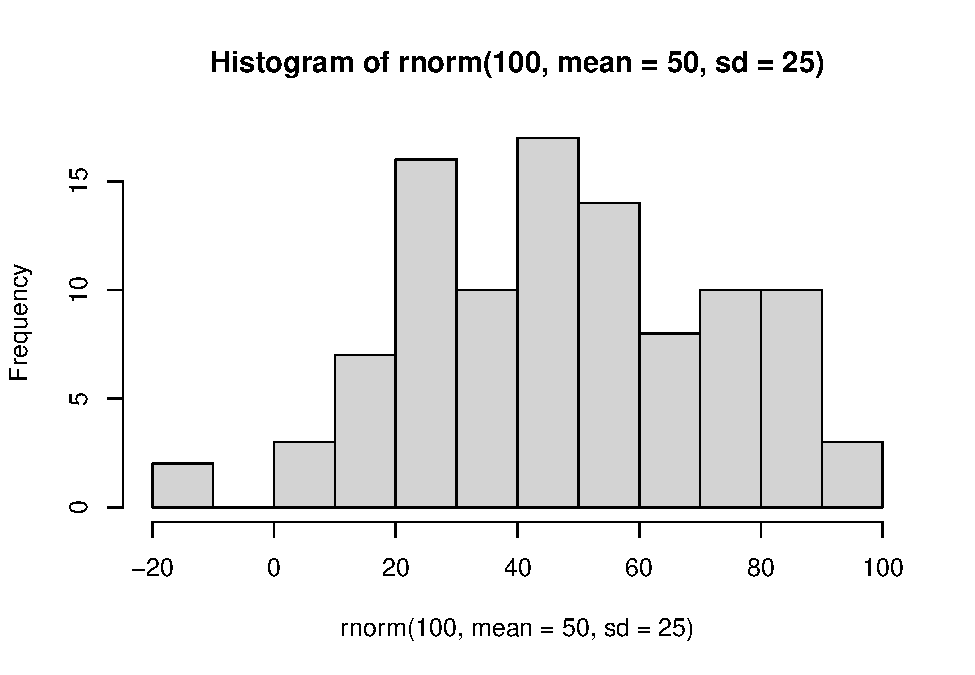
\includegraphics{quantrma_ex_files/figure-latex/unnamed-chunk-1-1.pdf}

You just made R sample 100 numbers, and then plot the results in a histogram. Pretty neat. We'll be doing some of this later in the course, where get R to make fake data for us, and then we learn to think about how data behaves under different kinds of assumptions.

For now, let's do something that might be a little bit more interesting\ldots what movies are going to be filming in NYC? It turns out that NYC makes a lot of data about a lot things open and free for anyone to download and look at. This is the NYC Open Data website: \url{https://opendata.cityofnewyork.us}. I searched through the data, and found a data file that lists the locations of film permits for shooting movies all throughout the Burroughs. There are multiple ways to load this data into R.

\begin{enumerate}
\def\labelenumi{\arabic{enumi}.}
\item
  If you have downloaded the \href{https://github.com/CrumpLab/statisticsLab/raw/master/RMarkdownsLab.zip}{RMarkdownsLab.zip} file, then you already have the data file in the data folder. Assuming you are working in your main directory (your .rmd file is saved in the main folder that contains both the data and template folders), then use the following commands to load the data.
\item
  If the above method doesn't work, you can try loading the data from the course website using:
\end{enumerate}

If you are having issues getting the data loaded, then talk to your lab instructor

\hypertarget{look-at-the-data}{%
\subsection{Look at the data}\label{look-at-the-data}}

You will be downloading and analyzing all kinds of data files this semester. We will follow the very same steps every time. The steps are to load the data, then look at it. You want to see what you've got.

In R-studio, you will now see a variable called \texttt{nyc\_films} in the top right-hand corner of the screen, in the environment tab. If you click this thing, it will show you the contents of the data in a new window. The data is stored in something we call a \texttt{data\ frame}. It's R lingo, for the thing that contains the data. Notice is a square, with rows going across, and columns going up and down. It looks kind of like an excel spreadsheet if you are familiar with Excel.

It's useful to know you can look at the data frame this way if you need to. But, this data frame is really big, it has 50,728 rows of data. That's a lot too much to look at.

\hypertarget{summarytools}{%
\subsubsection{summarytools}\label{summarytools}}

The summarytools packages give a quick way to summarize all of the data in a data frame. Here's how. When you run this code you will see the summary in the viewer on the bottom right hand side. There's a little browser button (arrow on top of little window) that you can click to expand and see the whole thing in a browser.

That is super helpful, but it's still a lot to look at. Because there is so much data here, it's pretty much mind-boggling to start thinking about what to do with it.

\hypertarget{make-plots-to-answer-questions}{%
\subsection{Make Plots to answer questions}\label{make-plots-to-answer-questions}}

Let's walk through a couple questions we might have about this data. We can see that there were 50,728 film permits made. We can also see that there are different columns telling us information about each of the film permits. For example, the \texttt{Borough} column lists the Borough for each request, whether it was made for: Manhattan, Brooklyn, Bronx, Queen's, or Staten Island. Now we can ask our first question, and learn how to do some plotting in R.

\hypertarget{where-are-the-most-film-permits-being-requested}{%
\subsubsection{Where are the most film permits being requested?}\label{where-are-the-most-film-permits-being-requested}}

Do you have any guesses? Is it Manhattan, or Brooklyn, of the Bronx? Or Queen's or Staten Island? We can find out by plotting the data using a bar plot. We just need to count how many film permits are made in each borough, and then make different bars represent the the counts.

First, we do the counting in R. Run the following code.

The above grouped the data by each of the five Borough's, and then counted the number of times each Borough occurred (using the \texttt{length} function). The result is a new variable called \texttt{count}. I chose to name this variable \texttt{count}. You can see that it is now displayed in the top-right hand corned in the environment tab. If you gave \texttt{count} a different name, like \texttt{muppets}, then it would be named what you called it.

If you click on the \texttt{counts} variable, you will see the five boroughs listed, along with the counts for how many film permits were requested in each Borough. These are the numbers that we want to plot in a graph.

We do the plot using a fantastic package called \texttt{ggplot2}. It is very powerful once you get the hand of it, and when you do, you will be able to make all sorts of interesting graphs. Here's the code to make the plot

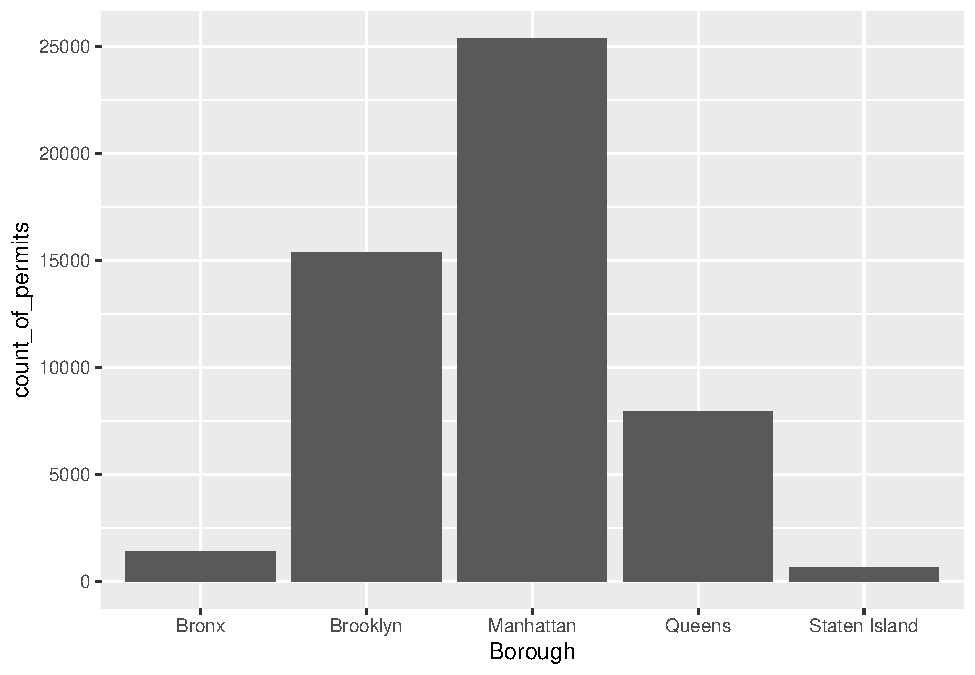
\includegraphics{quantrma_ex_files/figure-latex/1borough-1.pdf}

There it is, we're done here! We can easily look at this graph, and answer our question. Most of the film permits were requested in Manhattan, followed by Brooklyn, then Queen's, the Bronx, and finally Staten Island.

\hypertarget{what-kind-of-films-are-being-made-what-is-the-category}{%
\subsubsection{What kind of ``films'' are being made, what is the category?}\label{what-kind-of-films-are-being-made-what-is-the-category}}

We think you might be skeptical of what you are doing here, copying and pasting things. Soon you'll see just how fast you can do things by copying and pasting, and make a few little changes. Let's quickly ask another question about what kinds of films are being made. The column \texttt{Category}, gives us some information about that. Let's just copy paste the code we already made, and see what kinds of categories the films fall into. See if you can tell what I changed in the code to make this work, I'll do it all at once:

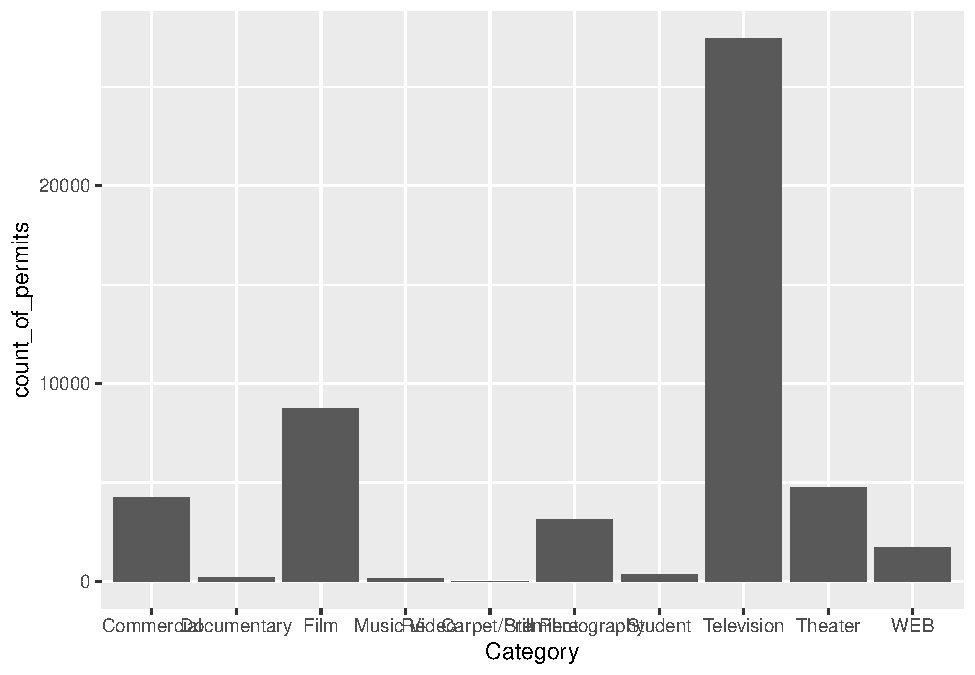
\includegraphics{quantrma_ex_files/figure-latex/1category-1.pdf}

OK, so this figure might look a bit weird because the labels on the bottom are running into each other. We'll fix that in a bit. First, let's notice the changes.

\begin{enumerate}
\def\labelenumi{\arabic{enumi}.}
\item
  I changed \texttt{Borough} to \texttt{Category}. That was the main thing
\item
  I left out a bunch of things from before. None of the \texttt{library()} commands are used again, and I didn't re-run the very early code to get the data. R already has those things in it's memory, so we don't need to do that first. If you ever clear the memory of R, then you will need to reload those things. First-things come first.
\end{enumerate}

Fine, so how do we fix the graph? Good question. To be honest, I don't know right now. I totally forgot how. But, I know ggplot2 can do this, and I'm going to Google it, right now. Then I'm going to find the answer, and use it here. The googling of your questions is a fine way to learn. It's what everybody does these days\ldots.{[}goes to Google\ldots{]}.

Found it, actually found a lot of ways to do this. The trick is to add the last line. I just copy-pasted it from the solution I found on \href{https://stackoverflow.com/questions/1330989/rotating-and-spacing-axis-labels-in-ggplot2}{stack overflow} (you will become friend's with stack overflow, there are many solutions there to all of your questions)

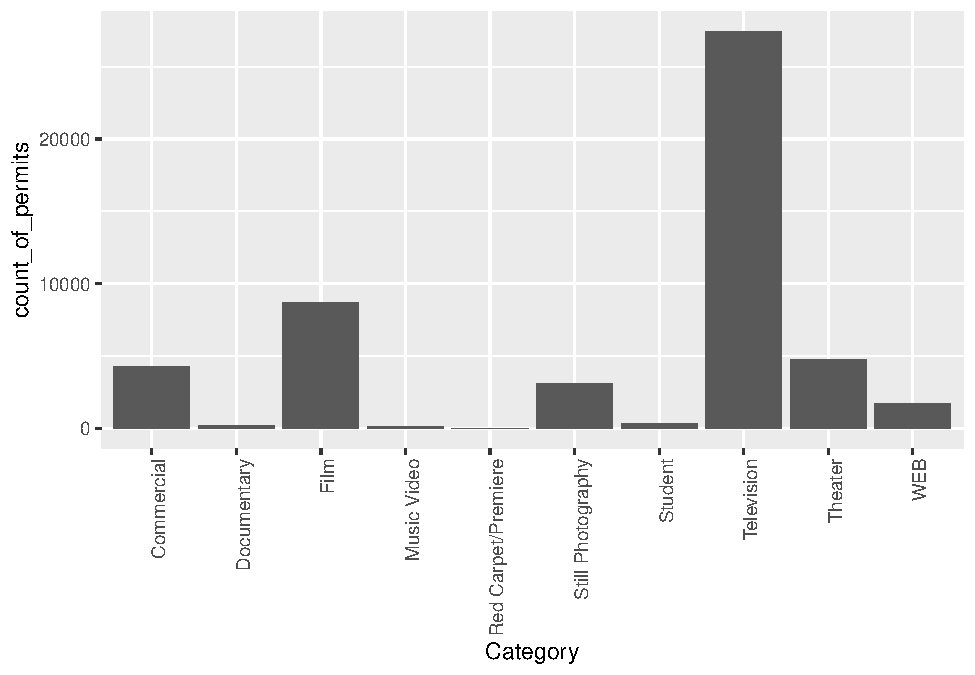
\includegraphics{quantrma_ex_files/figure-latex/1categoryB-1.pdf}

\hypertarget{ggplot2-basics}{%
\subsection{ggplot2 basics}\label{ggplot2-basics}}

Before we go further, I want to point out some basic properties of ggplot2, just to give you a sense of how it is working. This will make more sense in a few weeks, so come back here to remind yourself. We'll do just a bit a basics, and then move on to making more graphs, by copying and pasting.

The ggplot function uses layers. Layers you say? What are these layers? Well, it draws things from the bottom up. It lays down one layer of graphics, then you can keep adding on top, drawing more things. So the idea is something like: Layer 1 + Layer 2 + Layer 3, and so on. If you want Layer 3 to be Layer 2, then you just switch them in the code.

Here is a way of thinking about ggplot code

\begin{verbatim}
ggplot(name_of_data, aes(x = name_of_x_variable, y = name_of_y_variable)) +
    geom_layer()+
    geom_layer()+
    geom_layer()
\end{verbatim}

What I want you to focus on in the above description is the \(+\) signs. What we are doing with the plus signs is adding layers to plot. The layers get added in the order that they are written. If you look back to our previous code, you will see we add a \texttt{geom\_bar} layer, then we added another layer to change the rotation of the words on the x-axis. This is how it works.

BUT WAIT? How am I supposed to know what to add? This is nuts! We know. You're not supposed to know just yet, how could you? We'll give you lots of examples where you can copy and paste, and they will work. That's how you'll learn. If you really want to read the \href{https://ggplot2.tidyverse.org/reference/index.html}{help manual} you can do that too. It's on the ggplot2 website. This will become useful after you already know what you are doing, before that, it will probably just seem very confusing. However, it is pretty neat to look and \href{http://www.ggplot2-exts.org/gallery/}{see all of the different things you can do}, it's very powerful.

For now, let's the get the hang of adding things to the graph that let us change some stuff we might want to change. For example, how do you add a title? Or change the labels on the axes? Or add different colors, or change the font-size, or change the background? You can change all of these things by adding different lines to the existing code.

\hypertarget{ylab-changes-y-label}{%
\subsubsection{ylab() changes y label}\label{ylab-changes-y-label}}

The last graph had \texttt{count\_of\_permits} as the label on the y-axis. That doesn't look right. ggplot2 automatically took the label from the column, and made it be the name on the y-axis. We can change that by adding \texttt{ylab("what\ we\ want")}. We do this by adding a \(+\) to the last line, then adding \texttt{ylab()}

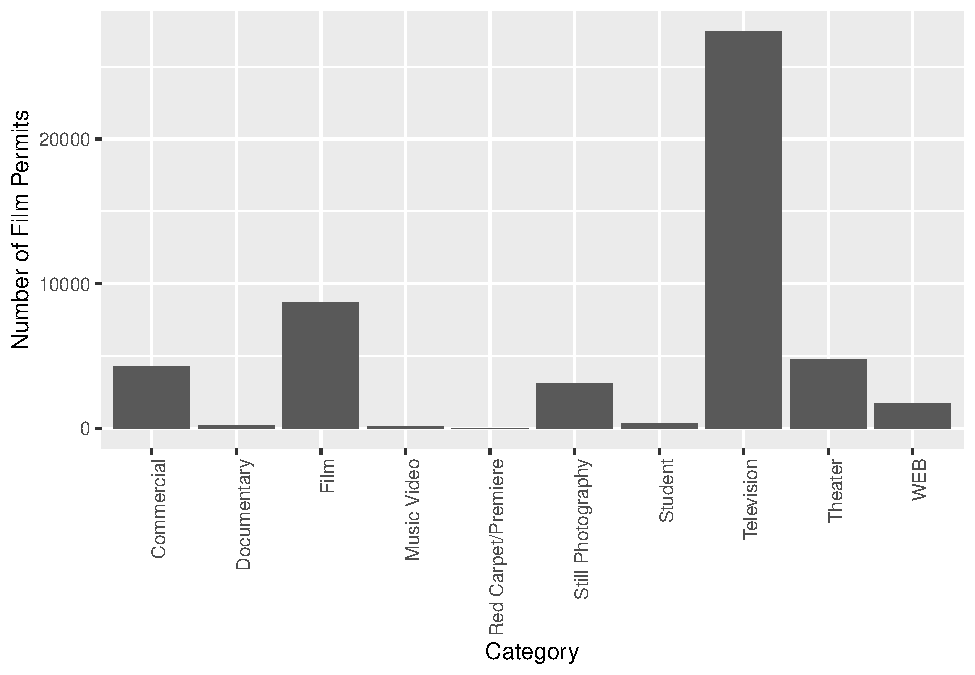
\includegraphics{quantrma_ex_files/figure-latex/1categoryC-1.pdf}

\hypertarget{xlab-changes-x-label}{%
\subsubsection{xlab() changes x label}\label{xlab-changes-x-label}}

Let's slightly modify the x label too:

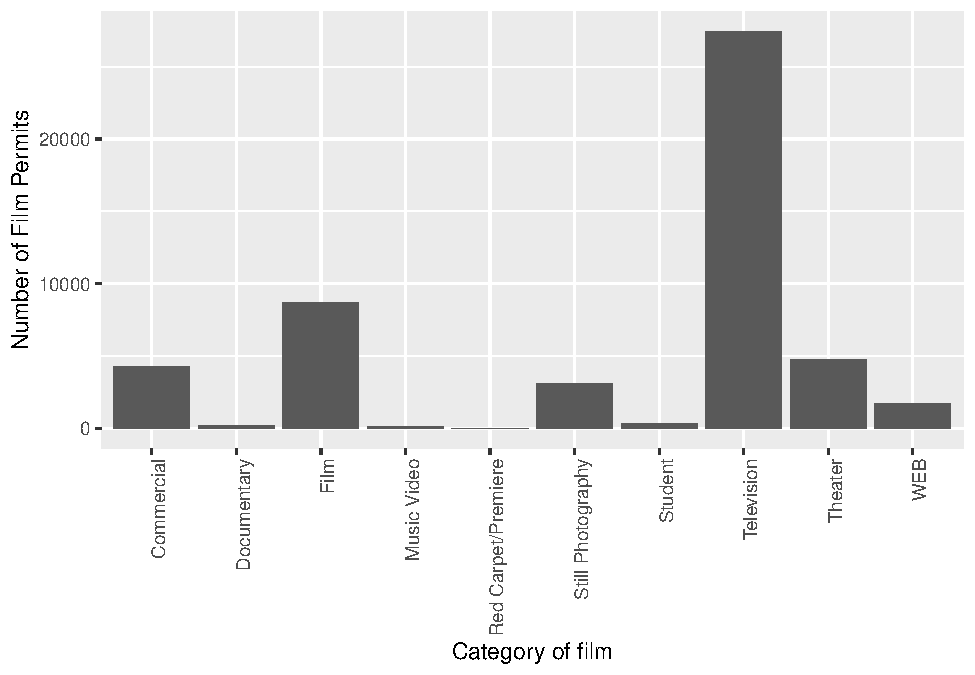
\includegraphics{quantrma_ex_files/figure-latex/1categoryD-1.pdf}

\hypertarget{ggtitle-adds-title}{%
\subsubsection{ggtitle() adds title}\label{ggtitle-adds-title}}

Let's give our graph a title

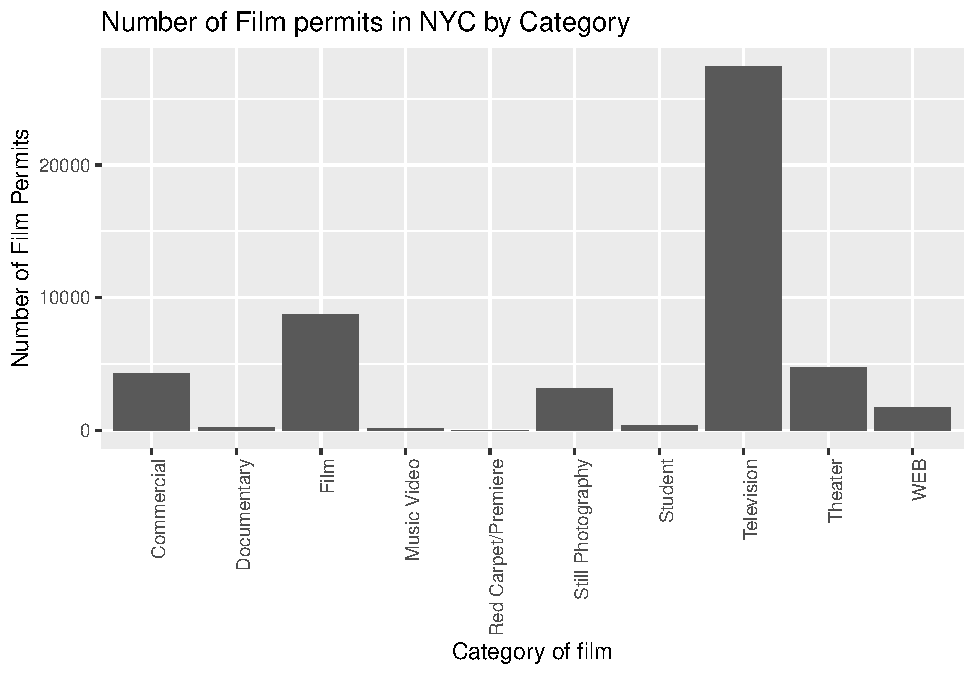
\includegraphics{quantrma_ex_files/figure-latex/1categoryE-1.pdf}

\hypertarget{color-adds-color}{%
\subsubsection{color adds color}\label{color-adds-color}}

Let's make the bars different colors. To do this, we add new code to the inside of the \texttt{aes()} part:

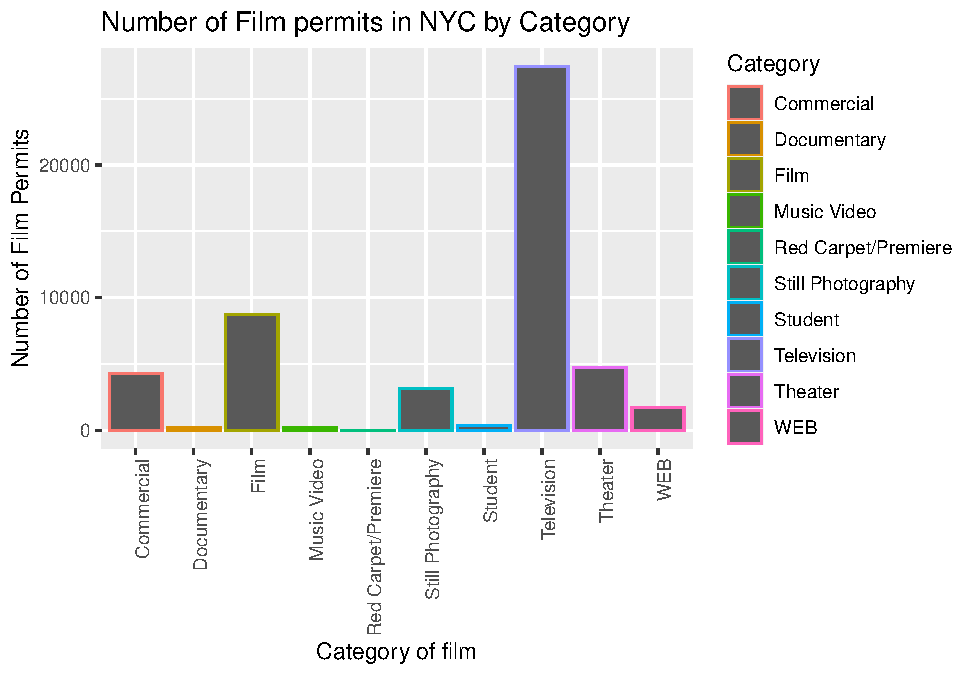
\includegraphics{quantrma_ex_files/figure-latex/1categoryF-1.pdf}

\hypertarget{fill-fills-in-color}{%
\subsubsection{fill fills in color}\label{fill-fills-in-color}}

Let's make the bars different colors. To do this, we add new code to the inside of the \texttt{aes()} part\ldots Notice I've started using new lines to make the code more readable.

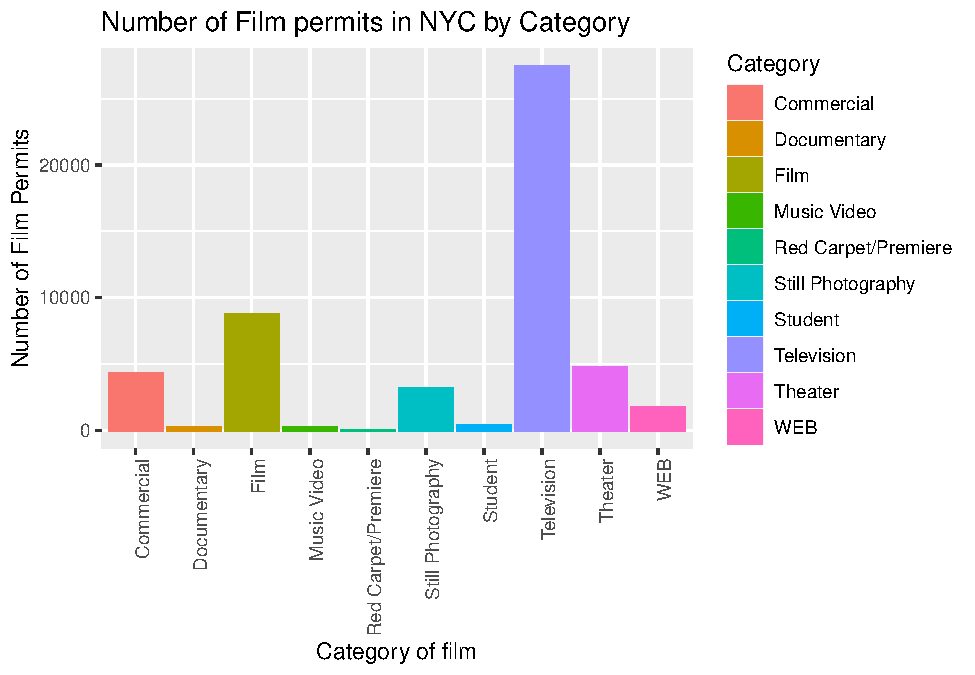
\includegraphics{quantrma_ex_files/figure-latex/1categoryG-1.pdf}

\hypertarget{get-rid-of-the-legend}{%
\subsubsection{get rid of the legend}\label{get-rid-of-the-legend}}

Sometimes you just don't want the legend on the side, to remove it add

\texttt{theme(legend.position="none")}

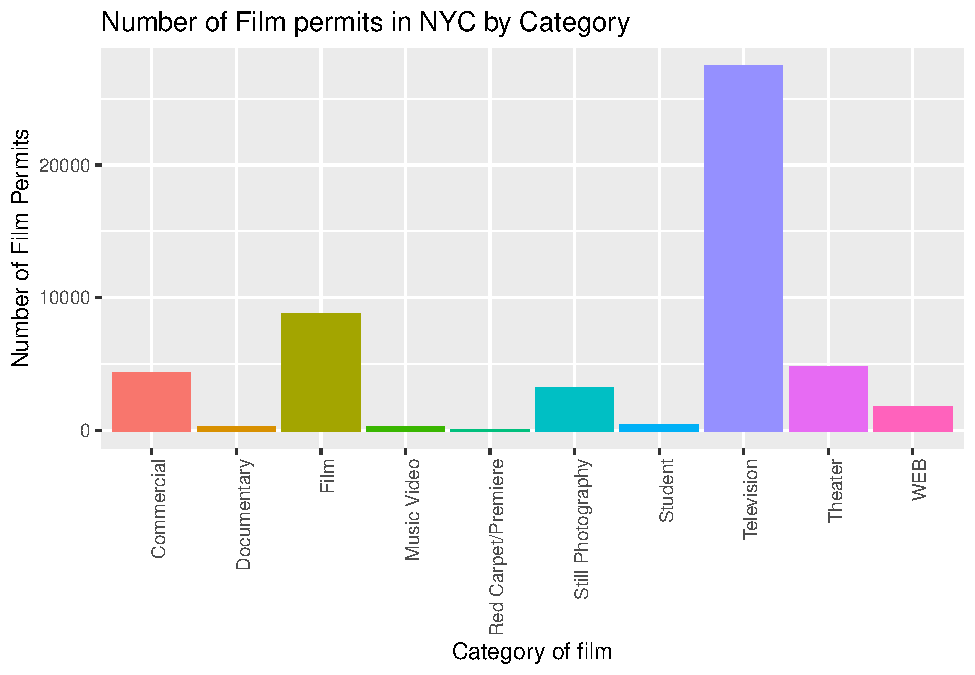
\includegraphics{quantrma_ex_files/figure-latex/1categoryH-1.pdf}

\hypertarget{theme_classic-makes-white-background}{%
\subsubsection{theme\_classic() makes white background}\label{theme_classic-makes-white-background}}

The rest is often just visual preference. For example, the graph above has this grey grid behind the bars. For a clean classic no nonsense look, use \texttt{theme\_classic()} to take away the grid.

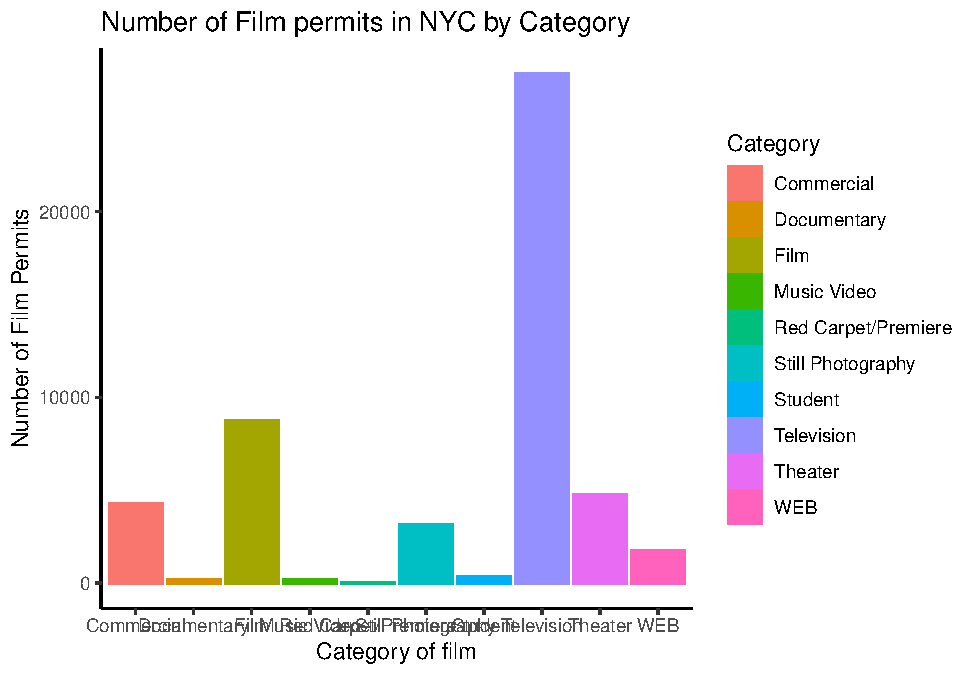
\includegraphics{quantrma_ex_files/figure-latex/1categoryI-1.pdf}

\hypertarget{sometimes-layer-order-matters}{%
\subsubsection{Sometimes layer order matters}\label{sometimes-layer-order-matters}}

Interesting, \texttt{theme\_classic()} is misbehaving a little bit. It looks like we have some of our layer out of order, let's re-order. I just moved \texttt{theme\_classic()} to just underneath the \texttt{geom\_bar()} line. Now everything get's drawn properly.

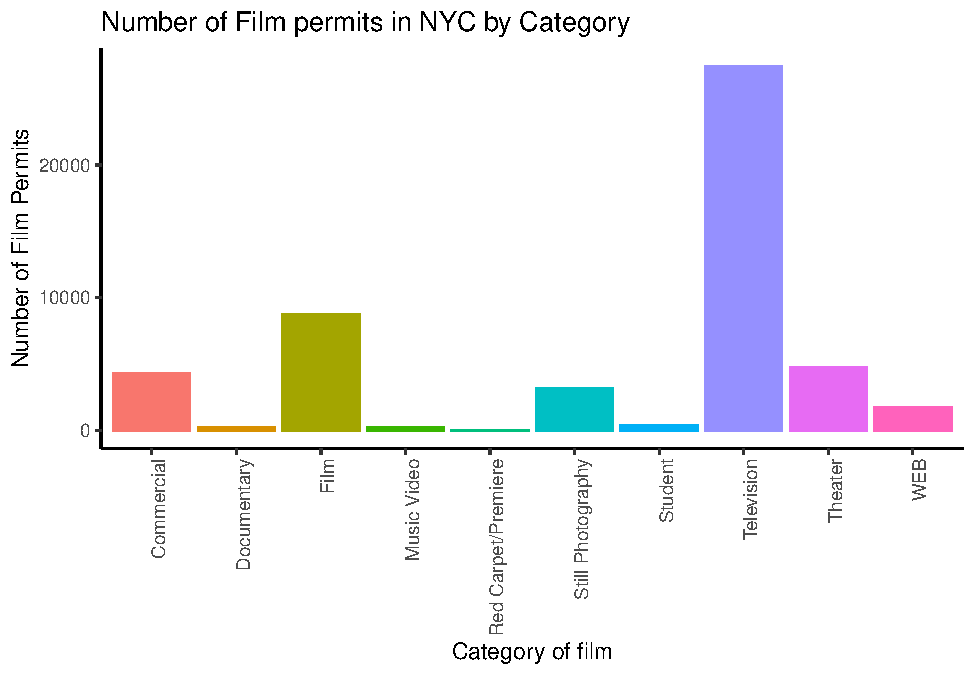
\includegraphics{quantrma_ex_files/figure-latex/1categoryJ-1.pdf}

\hypertarget{font-size}{%
\subsubsection{Font-size}\label{font-size}}

Changing font-size is often something you want to do. ggplot2 can do this in different ways. I suggest using the \texttt{base\_size} option inside \texttt{theme\_classic()}. You set one number for the largest font size in the graph, and everything else gets scaled to fit with that that first number. It's really convenient. Look for the inside of \texttt{theme\_classic()}

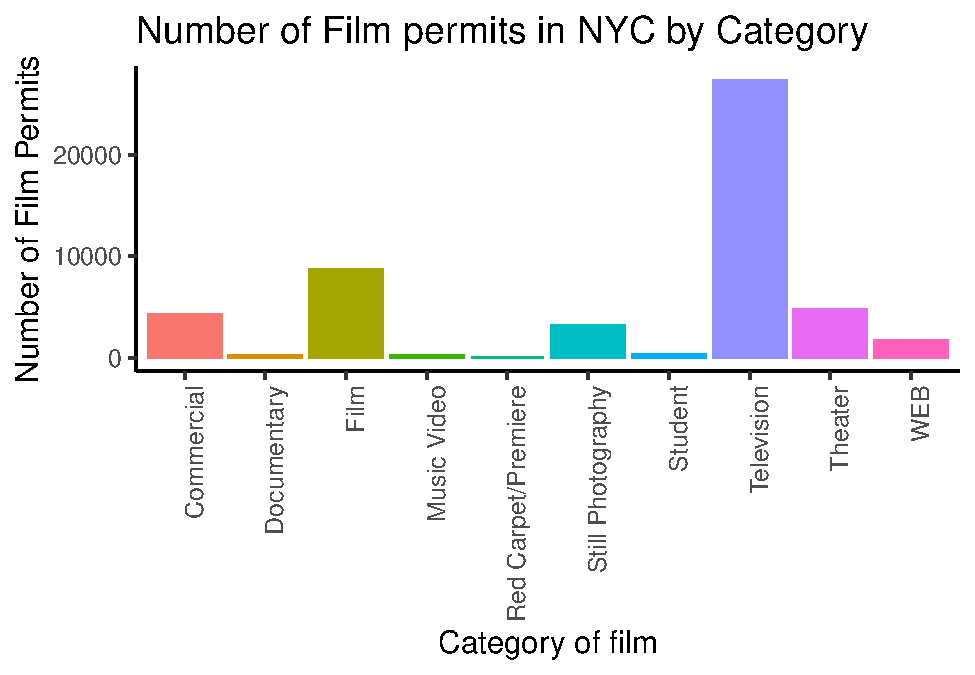
\includegraphics{quantrma_ex_files/figure-latex/1categoryK-1.pdf}
or make things small\ldots{} just to see what happens

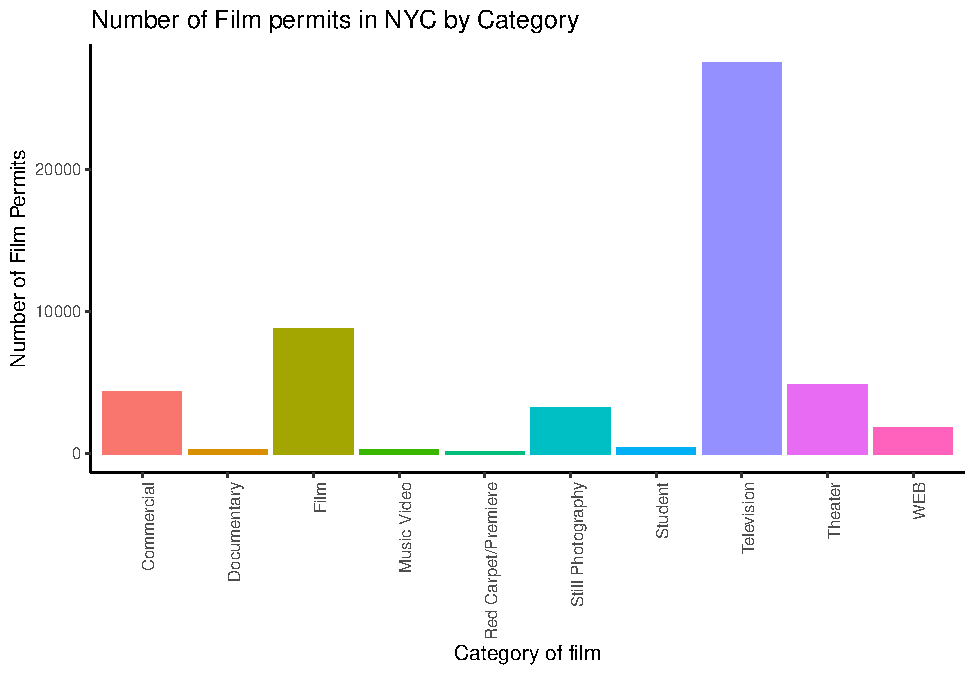
\includegraphics{quantrma_ex_files/figure-latex/1categoryL-1.pdf}

\hypertarget{ggplot2-summary}{%
\subsubsection{ggplot2 summary}\label{ggplot2-summary}}

That's enough of the ggplot2 basics for now. You will discover that many things are possible with ggplot2. It is amazing. We are going to get back to answering some questions about the data with graphs. But, now that we have built the code to make the graphs, all we need to do is copy-paste, and make a few small changes, and boom, we have our graph.

\hypertarget{more-questions-about-nyc-films}{%
\subsection{More questions about NYC films}\label{more-questions-about-nyc-films}}

\hypertarget{what-are-the-sub-categories-of-films}{%
\subsubsection{What are the sub-categories of films?}\label{what-are-the-sub-categories-of-films}}

Notice the \texttt{nyc\_films} data frame also has a column for \texttt{SubCategoryName}. Let's see what's going on there with a quick plot.

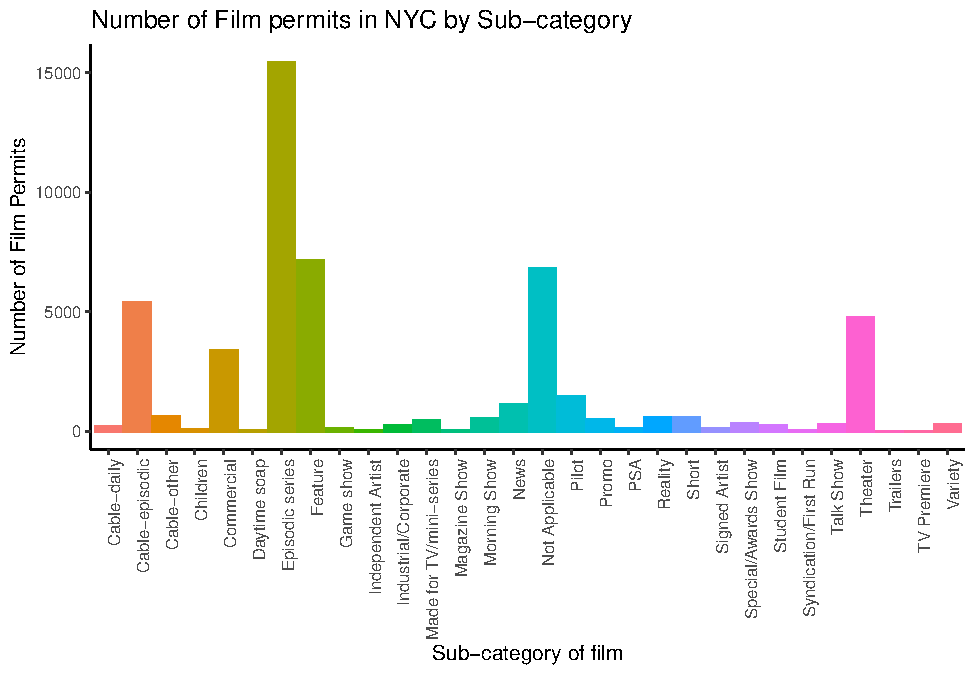
\includegraphics{quantrma_ex_files/figure-latex/1subcategory-1.pdf}

I guess ``episodic series'' are the most common. Using a graph like this gave us our answer super fast.

\hypertarget{categories-by-different-boroughs}{%
\subsubsection{Categories by different Boroughs}\label{categories-by-different-boroughs}}

Let's see one more really useful thing about ggplot2. It's called \texttt{facet\_wrap()}. It's an ugly word, but you will see that it is very cool, and you can do next-level-super-hero graph styles with \texttt{facet\_wrap} that other people can't do very easily.

Here's our question. We know that some films are made in different Boroughs, and that same films are made in different categories, but do different Boroughs have different patterns for the kinds of categories of films they request permits for? Are their more TV shows in Brooklyn? How do we find out? Watch, just like this:

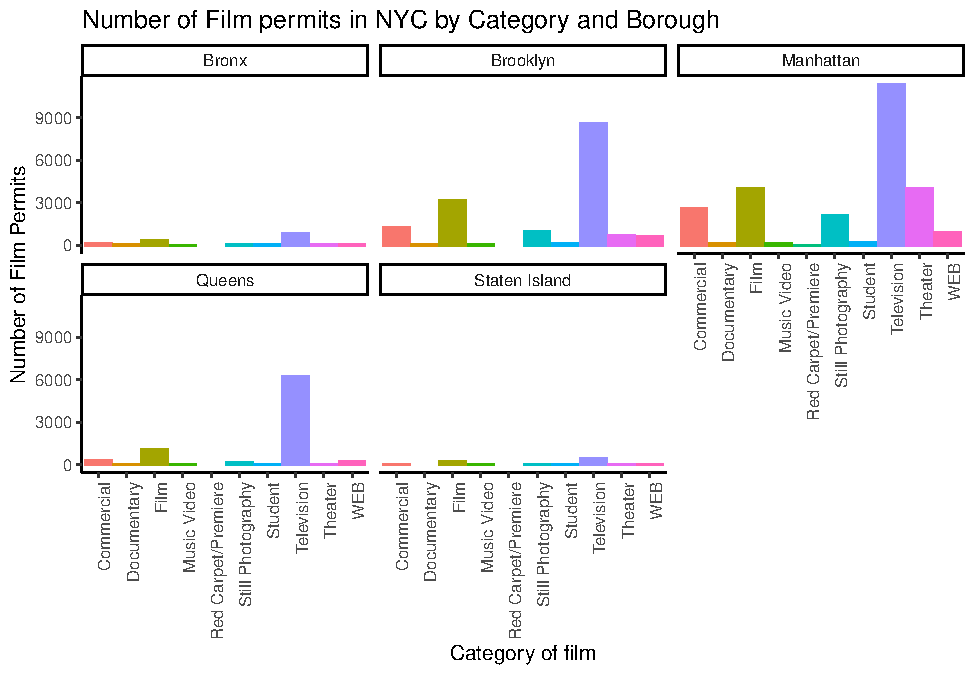
\includegraphics{quantrma_ex_files/figure-latex/1facetwrap-1.pdf}

We did two important things. First we added \texttt{Borough} and \texttt{Category} into the \texttt{group\_by()} function. This automatically gives separate counts for each category of film, for each Borough. Then we added \texttt{facet\_wrap(\textasciitilde{}Borough,\ ncol=3)} to the end of the plot, and it automatically drew us 5 different bar graphs, one for each Borough! That was fast. Imagine doing that by hand.

The nice thing about this is we can switch things around if we want. For example, we could do it this way by switching the \texttt{Category} with \texttt{Borough}, and facet-wrapping by Category instead of Borough like we did above. Do what works for you.

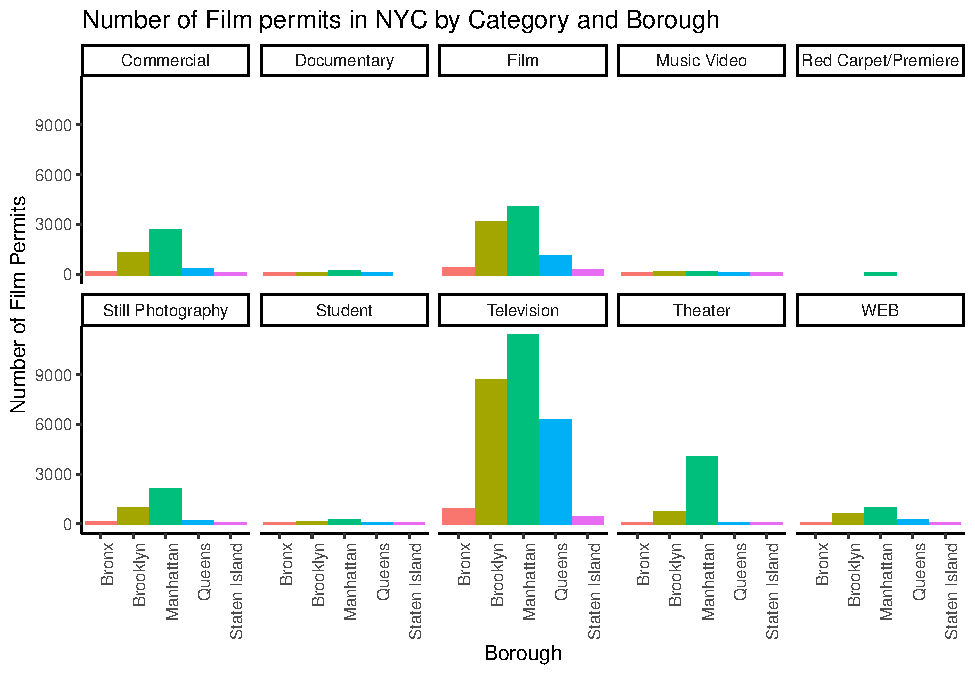
\includegraphics{quantrma_ex_files/figure-latex/1facetwrap2-1.pdf}

\hypertarget{gapminder-data}{%
\subsection{Gapminder Data}\label{gapminder-data}}

\url{https://www.gapminder.org} is an organization that collects some really interesting worldwide data. They also make cool visualization tools for looking at the data. There are many neat examples, and they have visualization tools built right into their website that you can play around with \url{https://www.gapminder.org/tools/}. That's fun check it out.

There is also an R package called \texttt{gapminder}. When you install this package, it loads in some of the data from gapminder, so we can play with it in R.

If you don't have the gapminder package installed, you can install it by running this code

Once the package is installed, you need to load the new library, like this. Then, you can put the \texttt{gapminder} data into a data frame, like we do here: \texttt{gapminder\_df}.

\hypertarget{look-at-the-data-frame}{%
\subsubsection{Look at the data frame}\label{look-at-the-data-frame}}

You can look at the data frame to see what is in it, and you can use \texttt{summarytools} again to view a summary of the data.

There are 1704 rows of data, and we see some columns for country, continent, year, life expectancy, population, and GDP per capita.

\hypertarget{asking-questions-with-the-gap-minder-data}{%
\subsection{Asking Questions with the gap minder data}\label{asking-questions-with-the-gap-minder-data}}

We will show you how to graph some the data to answer a few different kinds of questions. Then you will form your own questions, and see if you can answer them with ggplot2 yourself. All you will need to do is copy and paste the following examples, and change them up a little bit

\hypertarget{life-expectancy-histogram}{%
\subsubsection{Life Expectancy histogram}\label{life-expectancy-histogram}}

How long are people living all around the world according to this data set? There are many ways we could plot the data to find out. The first way is a histogram. We have many numbers for life expectancy in the column \texttt{lifeExp}. This is a big sample, full of numbers for 142 countries across many years. It's easy to make a histogram in ggplot to view the distribution:

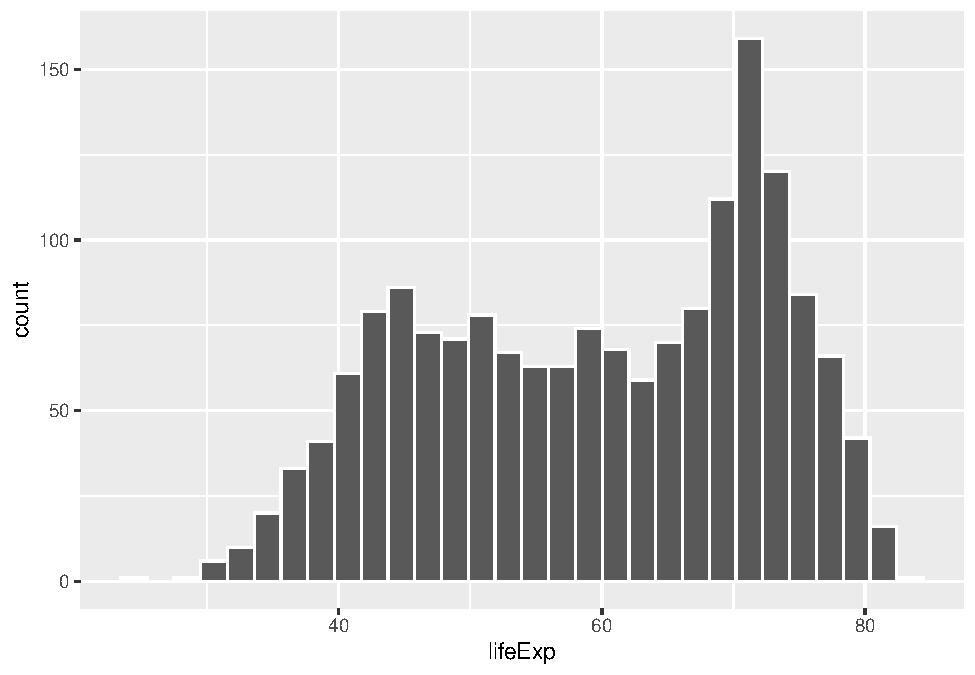
\includegraphics{quantrma_ex_files/figure-latex/1gapminder-1.pdf}

See, that was easy. Next, is a code block that adds more layers and settings if you wanted to modify parts of the graph:

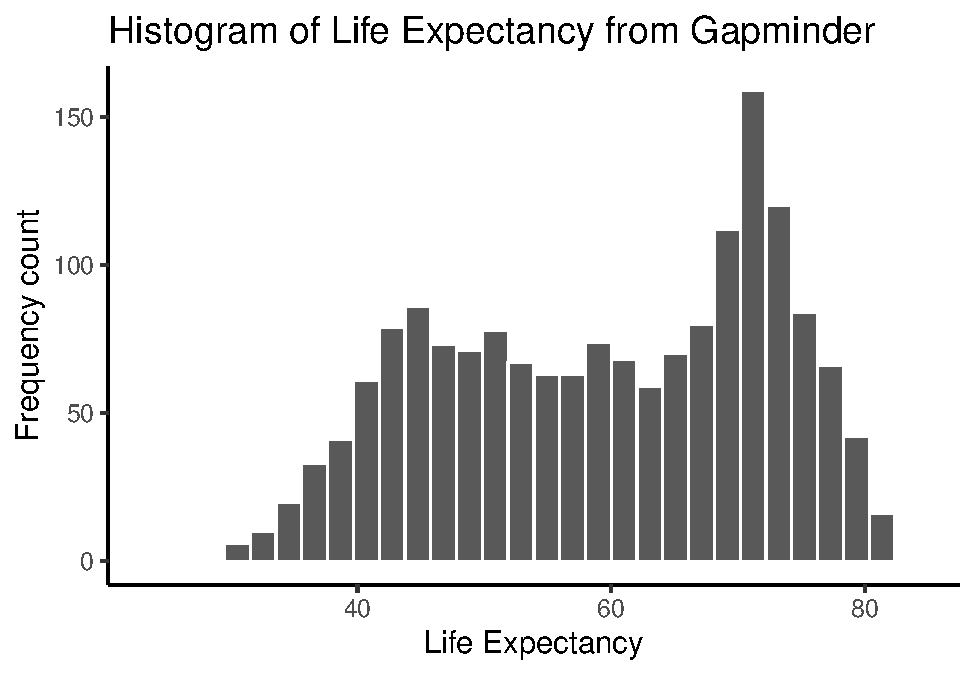
\includegraphics{quantrma_ex_files/figure-latex/1gapminderB-1.pdf}

The histogram shows a wide range of life expectancies, from below 40 to just over 80. Histograms are useful, they can show you what kinds of values happen more often than others.

One final thing about histograms in ggplot. You may want to change the bin size. That controls how wide or narrow, or the number of bars (how they split across the range), in the histogram. You need to set the \texttt{bins=} option in \texttt{geom\_histogram()}.

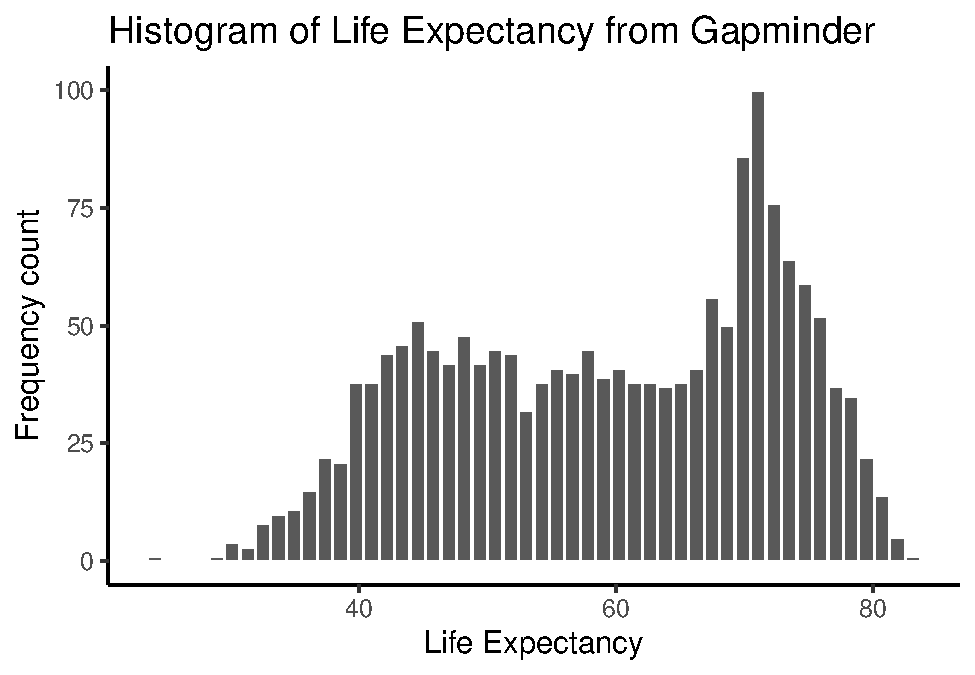
\includegraphics{quantrma_ex_files/figure-latex/1gapminderC-1.pdf}

See, same basic patter, but now breaking up the range into 50 little equal sized bins, rather than 30, which is the default. You get to choose what you want to do.

\hypertarget{life-expectancy-by-year-scatterplot}{%
\subsubsection{Life Expectancy by year Scatterplot}\label{life-expectancy-by-year-scatterplot}}

We can see we have data for life expectancy and different years. So, does worldwide life expectancy change across the years in the data set? As we go into the future, are people living longer?

Let's look at this using a scatter plot. We can set the x-axis to be year, and the y-axis to be life expectancy. Then we can use \texttt{geom\_point()} to display a whole bunch of dots, and then look at them. Here's the simple code:

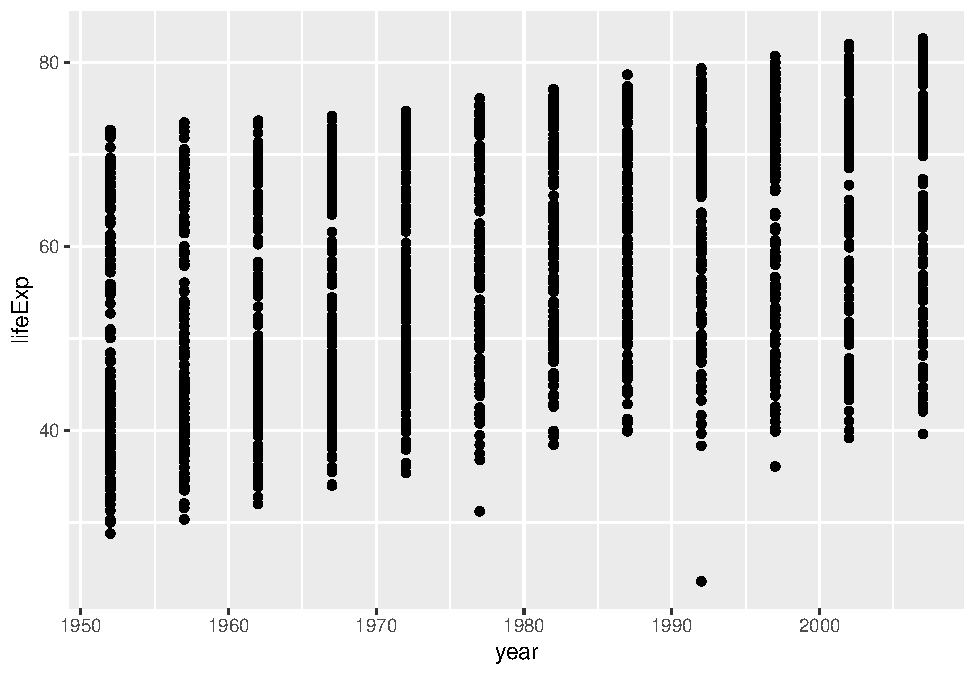
\includegraphics{quantrma_ex_files/figure-latex/1scatterplot-1.pdf}

Whoa, that's a lot of dots! Remember that each country is measured each year. So, the bands of dots you see, show the life expectancies for the whole range of countries within each year of the database. There is a big spread inside each year. But, on the whole it looks like groups of dots slowly go up over years.

\hypertarget{one-country-life-expectancy-by-year}{%
\subsubsection{One country, life expectancy by year}\label{one-country-life-expectancy-by-year}}

I'm (Matt) from Canada, so maybe I want to know if life expectancy for Canadians is going up over the years. To find out the answer for one country, we first need to split the full data set, into another smaller data set that only contains data for Canada. In other words, we want only the rows where the word ``Canada'' is found in the \texttt{country} column. We will use the \texttt{filter} function from \texttt{dplyr} for this:

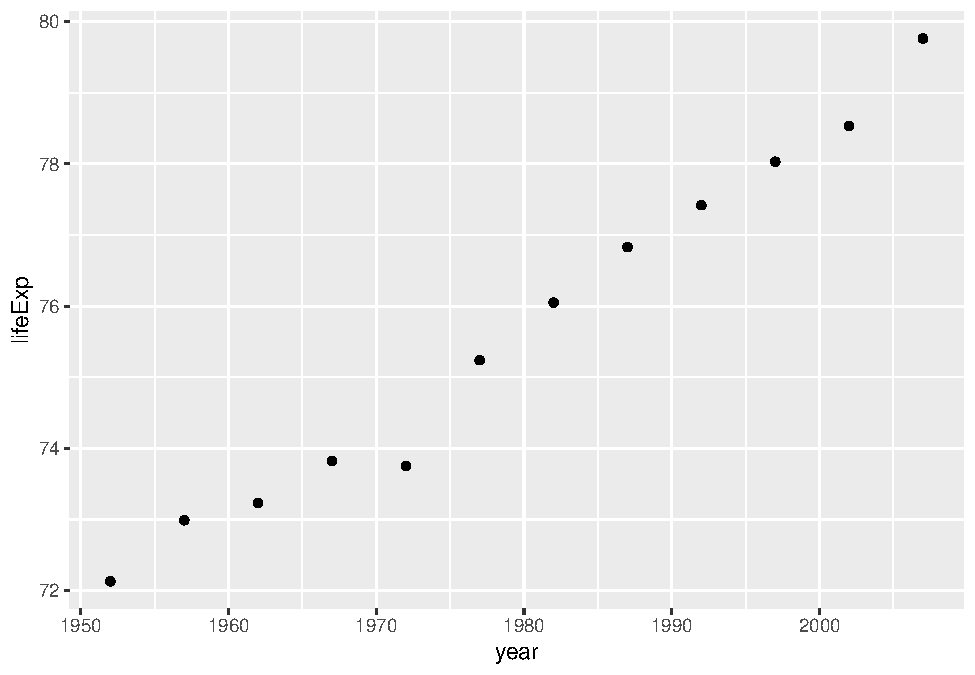
\includegraphics{quantrma_ex_files/figure-latex/1scatterB-1.pdf}

I would say things are looking good for Canadians, their life expectancy is going up over the years!

\hypertarget{multiple-countries-scatterplot}{%
\subsubsection{Multiple countries scatterplot}\label{multiple-countries-scatterplot}}

What if we want to look at a few countries altogether. We can do this too. We just change how we filter the data so more than one country is allowed, then we plot the data. We will also add some nicer color options and make the plot look pretty. First, the simple code:

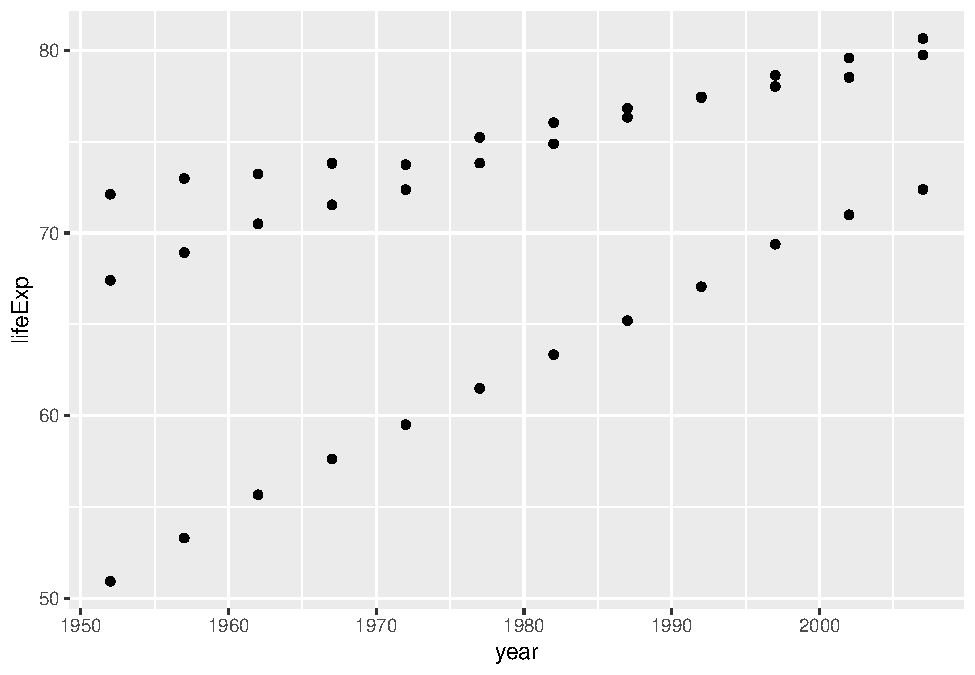
\includegraphics{quantrma_ex_files/figure-latex/1scatterC-1.pdf}

Nice, we can now see three sets of dots, but which are countries do they represent? Let's add a legend, and make the graph better looking.

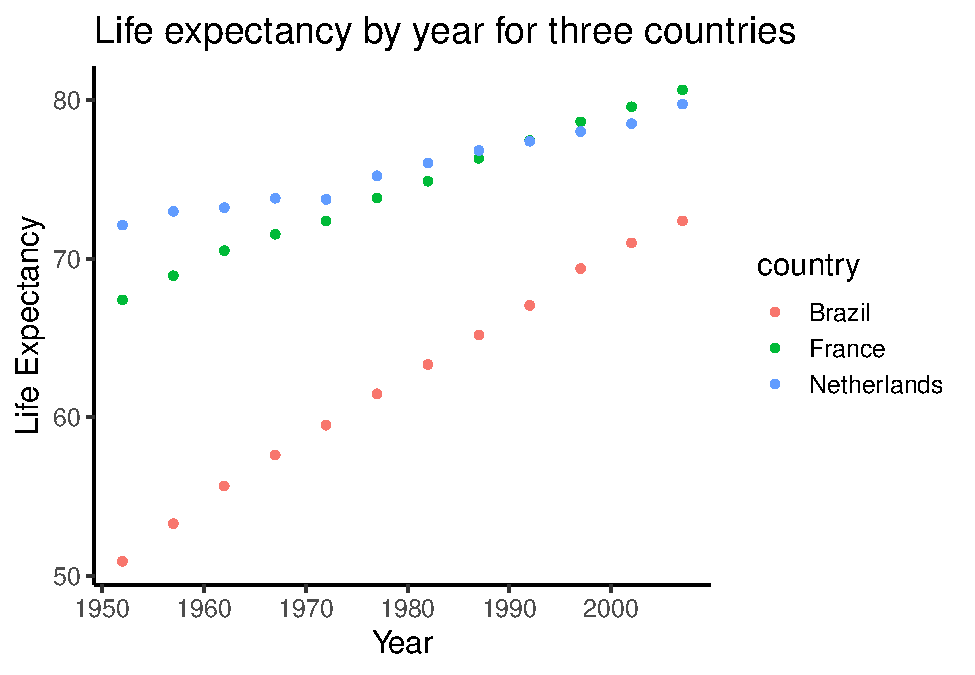
\includegraphics{quantrma_ex_files/figure-latex/1scatterD-1.pdf}

\hypertarget{geom_line-connecting-the-dots}{%
\subsubsection{geom\_line() connecting the dots}\label{geom_line-connecting-the-dots}}

We might also want to connect the dots with a line, to make it easier to see the connection! Remember, ggplot2 draws layers on top of layers. So, we add in a new \texttt{geom\_line()} layer.

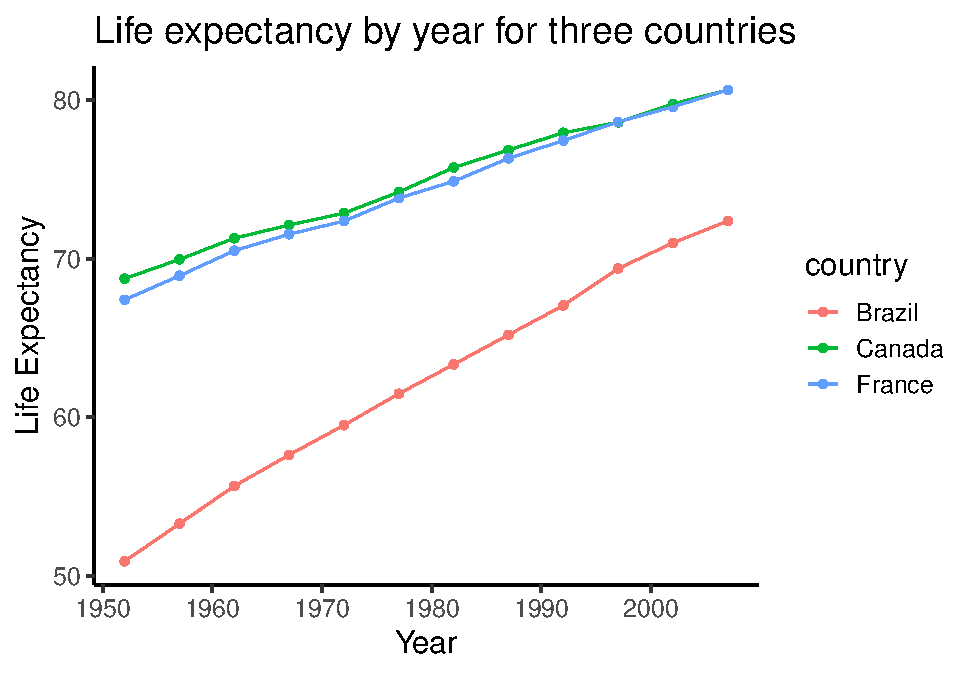
\includegraphics{quantrma_ex_files/figure-latex/1scatline-1.pdf}

\hypertarget{generalization-exercise}{%
\subsection{Generalization Exercise}\label{generalization-exercise}}

The following generalization exercise and writing assignment is also in your lab R Markdown document for this lab. Complete your work in that document and hand it in.

(1 point - Pass/Fail)

Use the code from above to attempt to solve the extra things we ask you do for this assignment. You generalization exercises are as follows:

\begin{enumerate}
\def\labelenumi{\arabic{enumi}.}
\item
  Make a graph plotting Life Expectancy by year for the five continents, using the \texttt{continent} factor. Make sure you change the title so it reads correctly
\item
  Make a graph plotting GDP per capita by year for the USA, Canada, and Mexico. Use the \texttt{gdpPercap} column for the GDP per capita data
\item
  Make a new graph plotting anything you are interested in using the gapminder dataset. It just needs to be a plot that we have not given an example for
\end{enumerate}

\hypertarget{writing-assignment}{%
\subsection{Writing assignment}\label{writing-assignment}}

Complete the writing assignment described in your R Markdown document for this lab. When you have finished everything. Knit the document and hand in your stuff (you can submit your .RMD file to blackboard if it does not knit.)

The question for this lab is a long answer question about histograms. Here is the question:

Describe what histograms are, how to interpret them, and what they are useful for. You should answer each of these questions:

The answers to each of these questions are worth .25 points each, for a total of 2 points

\begin{enumerate}
\def\labelenumi{\alph{enumi}.}
\tightlist
\item
  What do the bars on a histogram represent?
\item
  How many bars can a histogram have?
\item
  What do the heights of the bars tell you
\item
  What is on the x-axis and y-axis of a histogram
\item
  What does the tallest bar on a histogram tell you?
\item
  What does the shortest bar on a histogram tell you?
\item
  What are some uses for histograms, why would you want to look at a histogram of some numbers that you collected?
\item
  Imagine you had two histograms, one was very wide and spread out, the other was very narrow with a very tall peak. Which histogram would you expect to contain more consistent numbers (numbers that are close to each other), explain why.
\end{enumerate}

\textbf{Rubric}

General grading.

\begin{itemize}
\tightlist
\item
  You will receive 0 points for missing answers (say, if you do not answer question c, then you will receive 0 out .25 points for that question)
\item
  You must write in complete sentences. Point form sentences will be given 0 points.
\item
  Completely incorrect answers will receive 0 points. For example, if you incorrectly describe what the x and y-axes refer to, then you will receive 0 points for that question.
\item
  If your answer is generally correct but very difficult to understand and unclear you may receive half points for the question
\end{itemize}

\hypertarget{week-2-describing-data}{%
\chapter{Week 2: Describing Data}\label{week-2-describing-data}}

{
Describing comic sensibility is near impossible. It's sort of an abstract silliness, that sometimes the joke isn't the star.
---Dana Carvey
}

The purpose of this lab is to show you how to compute basic descriptive statistics, including measures of central tendency (mean, mode, median) and variation (range, variance, standard deviation).

\hypertarget{general-goals-1}{%
\section{General Goals}\label{general-goals-1}}

\begin{enumerate}
\def\labelenumi{\arabic{enumi}.}
\tightlist
\item
  Compute measures of central tendency using software
\item
  Compute measures of variation using software
\item
  Ask some questions of a data set using descriptive statistics
\end{enumerate}

\hypertarget{important-info-1}{%
\subsection{Important info}\label{important-info-1}}

We will be using data from the gapminder project. You can download a small snippet of the data in .csv format from this link (note this dataset was copied from the gapminder library for R) gapminder.csv. If you are using R, then you can install the gapminder package. This method is described later in the R section.

\hypertarget{r-1}{%
\section{R}\label{r-1}}

\hypertarget{descriptives-basics-in-r}{%
\subsection{Descriptives basics in R}\label{descriptives-basics-in-r}}

We learned in lecture and from the textbook that data we want to use ask and answer questions often comes with loads of numbers. Too many numbers to look at all at once. That's one reason we use descriptive statistics. To reduce the big set of numbers to one or two summary numbers that tell use something about all of the numbers. R can produce descriptive statistics for you in many ways. There are base functions for most of the ones that you want. We'll go over some R basics for descriptive statistics, and then use our new found skills to ask some questions about real data.

\hypertarget{making-numbers-in-r}{%
\subsubsection{Making numbers in R}\label{making-numbers-in-r}}

In order to do descriptive statistics we need to put some numbers in a variable. You can also do this using the \texttt{c()} command, which stands for combine

There a few other handy ways to make numbers. We can use \texttt{seq()} to make a sequence. Here's making the numbers from 1 to 100

We can repeat things, using rep. Here's making 10 5s, and 25 1s:

\begin{verbatim}
## [1] 10 10 10 10 10
\end{verbatim}

\begin{verbatim}
##  [1] 1 1 1 1 1 1 1 1 1 1 1 1 1 1 1 1 1 1 1 1 1 1 1 1 1
\end{verbatim}

\hypertarget{sum}{%
\subsubsection{Sum}\label{sum}}

Let's play with the number 1 to 100. First, let's use the \texttt{sum()} function to add them up

\begin{verbatim}
## [1] 5050
\end{verbatim}

\hypertarget{length}{%
\subsubsection{Length}\label{length}}

We put 100 numbers into the variable \texttt{one\_to\_one\_hundred}. We know how many numbers there are in there. How can we get R to tell us? We use \texttt{length()} for that.

\begin{verbatim}
## [1] 100
\end{verbatim}

\hypertarget{central-tendency}{%
\subsection{Central Tendency}\label{central-tendency}}

\hypertarget{mean}{%
\subsubsection{Mean}\label{mean}}

Remember the mean of some numbers is their sum, divided by the number of numbers. We can compute the mean like this:

\begin{verbatim}
## [1] 50.5
\end{verbatim}

Or, we could just use the \texttt{mean()} function like this:

\begin{verbatim}
## [1] 50.5
\end{verbatim}

\hypertarget{median}{%
\subsubsection{Median}\label{median}}

The median is the number in the exact middle of the numbers ordered from smallest to largest. If there are an even number of numbers (no number in the middle), then we take the number in between the two (decimal .5). Use the \texttt{median} function. There's only 3 numbers here. The middle one is 2, that should be the median

\begin{verbatim}
## [1] 2
\end{verbatim}

\hypertarget{mode}{%
\subsubsection{Mode}\label{mode}}

R does not a base function for the Mode. You would have to write one for yourself. Here is an example of writing your own mode function, and then using it. Note I searched how to do this on Google, and am using the mode defined by \href{https://stackoverflow.com/questions/2547402/is-there-a-built-in-function-for-finding-the-mode}{this answer on stack overflow}

Remember, the mode is the most frequently occurring number in the set. Below 1 occurs the most, so the mode will be one.

\begin{verbatim}
## [1] 1
\end{verbatim}

\hypertarget{variation}{%
\subsection{Variation}\label{variation}}

We often want to know how variable the numbers are. We are going to look at descriptive statistics to describe this such as the \textbf{range}, \textbf{variance}, the \textbf{standard deviation}, and a few others.

First, let's remind ourselves what variation looks like (it's when the numbers are different). We will sample 100 numbers from a normal distribution (don't worry about this yet), with a mean of 10, and a standard deviation of 5, and then make a histogram so we can see the variation around 10..

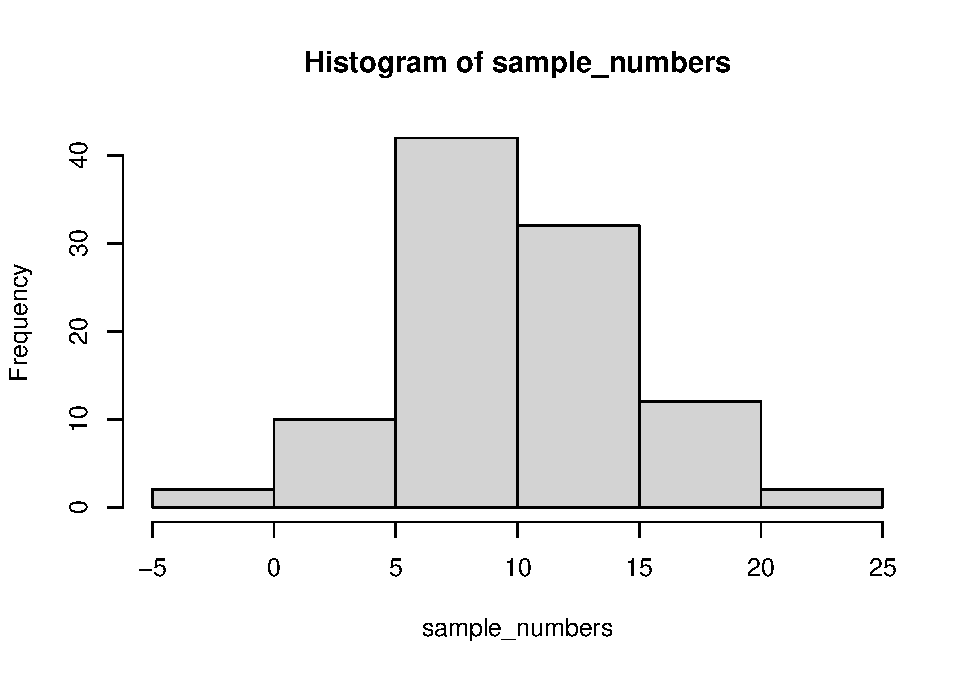
\includegraphics{quantrma_ex_files/figure-latex/unnamed-chunk-18-1.pdf}

\hypertarget{range}{%
\subsubsection{range}\label{range}}

The range is the minimum and maximum values in the set, we use the \texttt{range} function.

\begin{verbatim}
## [1] -2.023322 21.304595
\end{verbatim}

\hypertarget{var-variance}{%
\subsubsection{var = variance}\label{var-variance}}

We can find the sample variance using \texttt{var}. Note, divides by (n-1)

\begin{verbatim}
## [1] 21.07911
\end{verbatim}

\hypertarget{sd-standard-deviation}{%
\subsubsection{sd = standard deviation}\label{sd-standard-deviation}}

We find the sample standard deviation us SD. Note, divides by (n-1)

\begin{verbatim}
## [1] 4.5912
\end{verbatim}

Remember that the standard deviation is just the square root of the variance, see:

\begin{verbatim}
## [1] 4.5912
\end{verbatim}

\hypertarget{all-descriptives}{%
\subsubsection{All Descriptives}\label{all-descriptives}}

Let's put all of the descriptives and other functions so far in one place:

\begin{verbatim}
## [1] 992.8845
\end{verbatim}

\begin{verbatim}
## [1] 100
\end{verbatim}

\begin{verbatim}
## [1] 9.928845
\end{verbatim}

\begin{verbatim}
## [1] 9.603922
\end{verbatim}

\begin{verbatim}
## [1] 7.872911
\end{verbatim}

\begin{verbatim}
## [1]  0.908209 23.629800
\end{verbatim}

\begin{verbatim}
## [1] 23.955
\end{verbatim}

\begin{verbatim}
## [1] 4.894385
\end{verbatim}

\hypertarget{descriptives-by-conditions}{%
\subsection{Descriptives by conditions}\label{descriptives-by-conditions}}

Sometimes you will have a single variable with some numbers, and you can use the above functions to find the descriptives for that variable. Other times (most often in this course), you will have a big data frame of numbers, with different numbers in different conditions. You will want to find descriptive statistics for each the sets of numbers inside each of the conditions. Fortunately, this is where R really shines, it does it all for you in one go.

Let's illustrate the problem. Here I make a date frame with 10 numbers in each condition. There are 10 conditions, each labelled, A, B, C, D, E, F, G, H, I, J.

If you look at the \texttt{my\_df} data frame, you will see it has 100 rows, there are 10 rows for each condition with a label in the \texttt{conditions} column, and 10 scores for each condition in the \texttt{scores} column. What if you wanted to know the mean of the scores in each condition? You would want to find 10 means.

The slow way to do it would be like this:

\begin{verbatim}
## [1] 10.02365
\end{verbatim}

\begin{verbatim}
## [1] 10.63595
\end{verbatim}

\begin{verbatim}
## [1] 9.451351
\end{verbatim}

Nobody wants to do that! Not, me I stopped doing it that way, you should to.

\hypertarget{group_by-and-summarise}{%
\subsubsection{group\_by and summarise}\label{group_by-and-summarise}}

We can easily do everything all at once using the \texttt{group\_by} and \texttt{summarise} function from the \texttt{dplyr} package. Just watch

\begin{verbatim}
## # A tibble: 10 x 2
##    conditions means
##    <chr>      <dbl>
##  1 A          10.0 
##  2 B          10.6 
##  3 C           9.45
##  4 D          10.8 
##  5 E          10.5 
##  6 F          10.3 
##  7 G           7.10
##  8 H          10.0 
##  9 I           8.89
## 10 J          12.8
\end{verbatim}

A couple things now. First, the print out of this was ugly. Let's fix that. we put the results of our code into a new variable, then we use \texttt{knitr::kable} to print it out nicely when we \texttt{knit} the document

\begin{tabular}{l|r}
\hline
conditions & means\\
\hline
A & 10.023654\\
\hline
B & 10.635952\\
\hline
C & 9.451351\\
\hline
D & 10.764120\\
\hline
E & 10.502361\\
\hline
F & 10.310111\\
\hline
G & 7.101817\\
\hline
H & 10.045395\\
\hline
I & 8.887561\\
\hline
J & 12.841569\\
\hline
\end{tabular}

\hypertarget{multiple-descriptives}{%
\subsubsection{multiple descriptives}\label{multiple-descriptives}}

The best thing about the \texttt{dplyr} method, is that we can add more than one function, and we'll get more than one summary returned, all in a nice format, let's add the standard deviation:

\begin{tabular}{l|r|r}
\hline
conditions & means & sds\\
\hline
A & 10.023654 & 4.604208\\
\hline
B & 10.635952 & 3.281958\\
\hline
C & 9.451351 & 5.273949\\
\hline
D & 10.764120 & 5.479498\\
\hline
E & 10.502361 & 4.083631\\
\hline
F & 10.310111 & 6.036790\\
\hline
G & 7.101817 & 4.854278\\
\hline
H & 10.045395 & 4.476087\\
\hline
I & 8.887561 & 5.824516\\
\hline
J & 12.841569 & 5.131564\\
\hline
\end{tabular}

We'll add the min and the max too:

\begin{tabular}{l|r|r|r|r}
\hline
conditions & means & sds & min & max\\
\hline
A & 10.023654 & 4.604208 & 4.1653804 & 19.16399\\
\hline
B & 10.635952 & 3.281958 & 4.6025178 & 16.23753\\
\hline
C & 9.451351 & 5.273949 & 2.5979282 & 16.09684\\
\hline
D & 10.764120 & 5.479498 & 2.2711705 & 17.44698\\
\hline
E & 10.502361 & 4.083631 & 3.7584837 & 16.07643\\
\hline
F & 10.310111 & 6.036790 & 0.3710595 & 19.24557\\
\hline
G & 7.101817 & 4.854278 & -2.2646016 & 17.28045\\
\hline
H & 10.045395 & 4.476087 & 4.1255610 & 19.25093\\
\hline
I & 8.887561 & 5.824516 & 1.2089960 & 18.12876\\
\hline
J & 12.841569 & 5.131564 & 5.4196560 & 23.74913\\
\hline
\end{tabular}

\hypertarget{describing-gapminder}{%
\subsection{Describing gapminder}\label{describing-gapminder}}

Now that we know how to get descriptive statistics from R, we cam do this will some real data. Let's quickly ask a few question about the gapminder data.

Note: The above code will only work if you have installed the gapminder package. Make sure you are connected to the internet, then choose the Packages tab from the bottom right panel, and choose install. Thens search for gapminder, choose it, and install it.

\hypertarget{what-are-some-descriptive-for-life-expectancy-by-continent}{%
\subsubsection{What are some descriptive for Life expectancy by continent?}\label{what-are-some-descriptive-for-life-expectancy-by-continent}}

Copy the code from the last part of descriptives using \texttt{dplyr}, then change the names like this:

\begin{tabular}{l|r|r|r|r}
\hline
continent & means & sds & min & max\\
\hline
Africa & 48.86533 & 9.150210 & 23.599 & 76.442\\
\hline
Americas & 64.65874 & 9.345088 & 37.579 & 80.653\\
\hline
Asia & 60.06490 & 11.864532 & 28.801 & 82.603\\
\hline
Europe & 71.90369 & 5.433178 & 43.585 & 81.757\\
\hline
Oceania & 74.32621 & 3.795611 & 69.120 & 81.235\\
\hline
\end{tabular}

\hypertarget{generalization-exercise-1}{%
\subsection{Generalization Exercise}\label{generalization-exercise-1}}

(1 point - Pass/Fail)

Complete the generalization exercise described in your R Markdown document for this lab.

\begin{enumerate}
\def\labelenumi{\arabic{enumi}.}
\item
  What is the mean, standard deviation, minimum and maximum life expectancy for all the gapminder data (across all the years and countries). Hint: do not use \texttt{group\_by}
\item
  What is the mean, standard deviation, minimum and maximum life expectancy for all of the continents in 2007, the most recent year in the dataset. Hint: add another pipe using \texttt{filter(year==2007)\ \%\textgreater{}\%}
\end{enumerate}

\hypertarget{writing-assignment-1}{%
\subsection{Writing assignment}\label{writing-assignment-1}}

(2 points - Graded)

Complete the writing assignment described in your R Markdown document for this lab. When you have finished everything. Knit the document and hand in your stuff (you can submit your .RMD file to blackboard if it does not knit.)

Your writing assignment is to answer these questions in full sentences using simple plain langauge:

\begin{enumerate}
\def\labelenumi{\arabic{enumi}.}
\tightlist
\item
  Define the mode.
\item
  Explain what would need to happen in order for a set of numbers to have two modes
\item
  Define the median
\item
  Define the mean
\item
  Define the range
\item
  When calculating the standard deviation, explain what the difference scores represent
\item
  Explain why the difference scores are squared when calculating the standard deviation
\item
  If one set of numbers had a standard deviation of 5, and another had a standard deviation of 10, which set of numbers would have greater variance, explain why.
\end{enumerate}

\textbf{Rubric}

General grading.

\begin{itemize}
\tightlist
\item
  You will receive 0 points for missing answers (say, if you do not answer question c, then you will receive 0 out .25 points for that question)
\item
  You must write in complete sentences. Point form sentences will be given 0 points.
\item
  Completely incorrect answers will receive 0 points.
\item
  If your answer is generally correct but very difficult to understand and unclear you may receive half points for the question
\end{itemize}

\hypertarget{week-3-correlation-and-causation}{%
\chapter{Week 3: Correlation and Causation}\label{week-3-correlation-and-causation}}

{
If \ldots{} we choose a group of social phenomena with no antecedent knowledge of the causation or absence of causation among them, then the calculation of correlation coefficients, total or partial, will not advance us a step toward evaluating the importance of the causes at work.
---Sir Ronald Fisher
}

In lecture and in the textbook, we have been discussing the idea of correlation. This is the idea that two things that we measure can be somehow related to one another. For example, your personal happiness, which we could try to measure say with a questionnaire, might be related to other things in your life that we could also measure, such as number of close friends, yearly salary, how much chocolate you have in your bedroom, or how many times you have said the word Nintendo in your life. Some of the relationships that we can measure are meaningful, and might reflect a causal relationship where one thing causes a change in another thing. Some of the relationships are spurious, and do not reflect a causal relationship.

In this lab you will learn how to compute correlations between two variables in software, and then ask some questions about the correlations that you observe.

\hypertarget{general-goals-2}{%
\section{General Goals}\label{general-goals-2}}

\begin{enumerate}
\def\labelenumi{\arabic{enumi}.}
\tightlist
\item
  Compute Pearson's r between two variables using software
\item
  Discuss the possible meaning of correlations that you observe
\end{enumerate}

\hypertarget{important-info-2}{%
\subsection{Important Info}\label{important-info-2}}

We use data from the \href{http://worldhappiness.report}{World Happiness Report}. A .csv of the data can be found here: WHR2018.csv

\hypertarget{r-2}{%
\section{R}\label{r-2}}

In this lab we use explore to explore correlations between any two variables, and also show how to do a regression line. There will be three main parts. Getting R to compute the correlation, and looking at the data using scatter plots. We'll look at some correlations from the World Happiness Report. Then you'll look at correlations using data we collect from ourselves. It will be fun.

\hypertarget{cor-for-correlation}{%
\subsection{cor for correlation}\label{cor-for-correlation}}

R has the \texttt{cor} function for computing Pearson's r between any two variables. In fact this same function computes other versions of correlation, but we'll skip those here. To use the function you just need two variables with numbers in them like this:

\begin{verbatim}
## [1] 0.76539
\end{verbatim}

Well, that was easy.

\hypertarget{scatterplots}{%
\subsubsection{scatterplots}\label{scatterplots}}

Let's take our silly example, and plot the data in a scatter plot using ggplot2, and let's also return the correlation and print it on the scatter plot. Remember, ggplot2 wants the data in a data.frame, so we first put our x and y variables in a data frame.

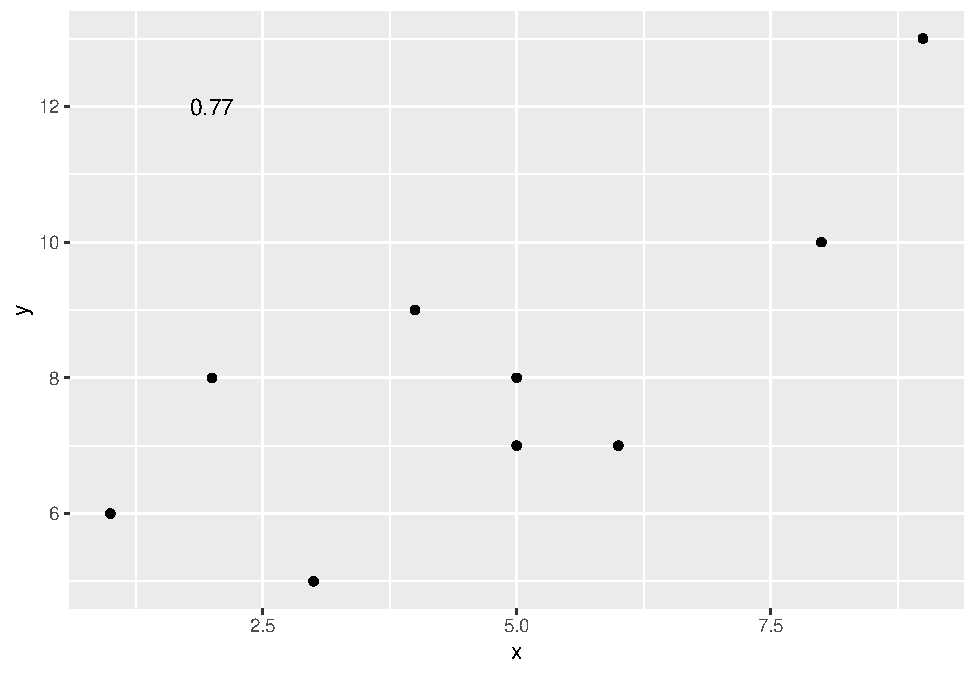
\includegraphics{quantrma_ex_files/figure-latex/unnamed-chunk-33-1.pdf}

Wow, we're moving fast here.

\hypertarget{lots-of-scatterplots}{%
\subsubsection{lots of scatterplots}\label{lots-of-scatterplots}}

Before we move on to real data, let's look at some fake data first. Often we will have many measures of X and Y, split between a few different conditions, for example, A, B, C, and D. Let's make some fake data for X and Y, for each condition A, B, C, and D, and then use facet\_wrapping to look at four scatter plots all at once

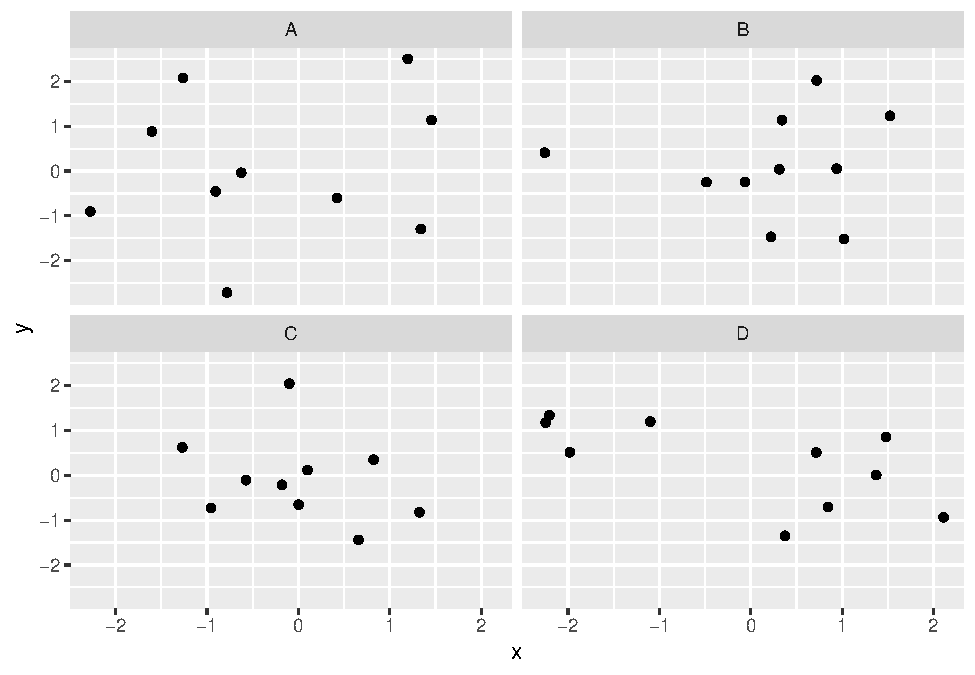
\includegraphics{quantrma_ex_files/figure-latex/unnamed-chunk-34-1.pdf}

\hypertarget{computing-the-correlations-all-at-once}{%
\subsubsection{computing the correlations all at once}\label{computing-the-correlations-all-at-once}}

We've seen how we can make four graphs at once. Facet\_wrap will always try to make as many graphs as there are individual conditions in the column variable. In this case there are four, so it makes four.

Notice, the scatter plots don't show the correlation (r) values. Getting these numbers on there is possible, but we have to calculate them first. We'll leave it to you to Google how to do this, if it's something you want to do. Instead, what we will do is make a table of the correlations in addition to the scatter plot. We again use \texttt{dplyr} to do this:

OK, we are basically ready to turn to some real data and ask if there are correlations between interesting variables\ldots You will find that there are some\ldots{} But before we do that, we do one more thing. This will help you become a little bit more skeptical of these ``correlations''.

\hypertarget{chance-correlations}{%
\subsubsection{Chance correlations}\label{chance-correlations}}

As you learned from the textbook. We can find correlations by chance alone, even when there is no true correlation between the variables. For example, if we sampled randomly into x, and then sampled some numbers randomly into y. We know they aren't related, because we randomly sampled the numbers. However, doing this creates some correlations some of the time just by chance. You can demonstrate this to yourself with the following code. It's a repeat of what we already saw, jut with a few more conditions added. Let's look at 20 conditions, with random numbers for x and y in each. For each, sample size will be 10. We'll make the fake data, then make a big graph to look at all. And, even though we get to regression later in the lab, I'll put the best fit line onto each scatter plot, so you can ``see the correlations''.

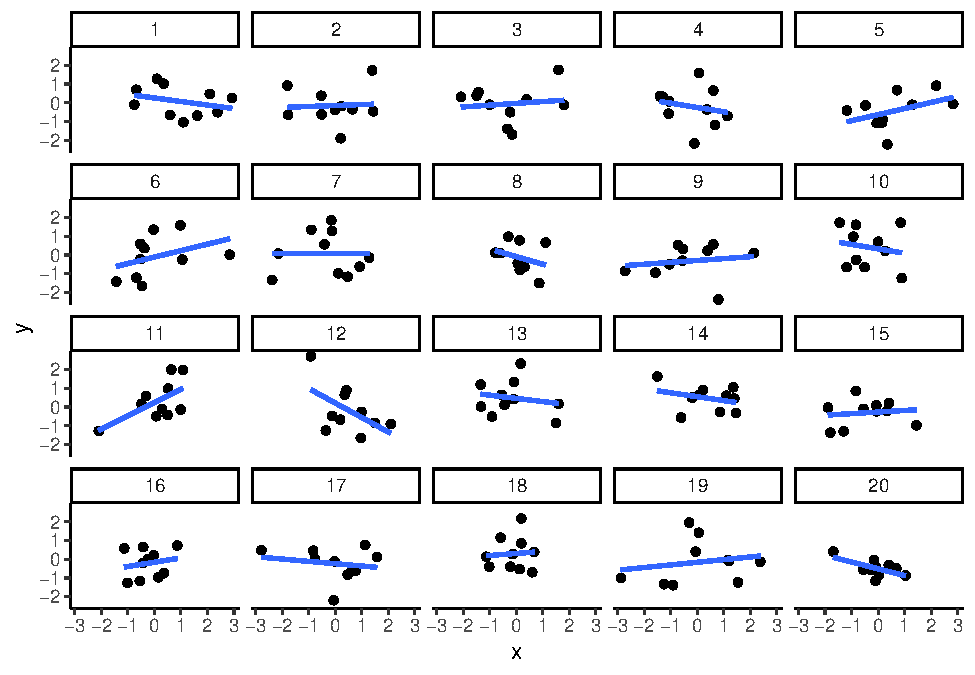
\includegraphics{quantrma_ex_files/figure-latex/unnamed-chunk-35-1.pdf}

You can see that the slope of the blue line is not always flat. Sometimes it looks like there is a correlation, when we know there shouldn't be. You can keep re-doing this graph, by re-knitting your R Markdown document, or by pressing the little green play button. This is basically you simulating the outcomes as many times as you press the button.

The point is, now you know you can find correlations by chance. So, in the next section, you should always wonder if the correlations you find reflect meaningful association between the x and y variable, or could have just occurred by chance.

\hypertarget{world-happiness-report}{%
\subsection{World Happiness Report}\label{world-happiness-report}}

Let's take a look at some correlations in real data. We are going to look at responses to a questionnaire about happiness that was sent around the world, from the \href{http://worldhappiness.report}{world happiness report}

\hypertarget{load-the-data}{%
\subsubsection{Load the data}\label{load-the-data}}

We load the data into a data frame. Reminder, the following assumes that you have downloaded the \href{https://github.com/CrumpLab/statisticsLab/raw/master/RMarkdownsLab.zip}{RMarkdownsLab.zip} file which contains the data file in the data folder.

You can also load the data using the following URL

\hypertarget{look-at-the-data-1}{%
\subsubsection{Look at the data}\label{look-at-the-data-1}}

You should be able to see that there is data for many different countries, across a few different years. There are lots of different kinds of measures, and each are given a name. I'll show you some examples of asking questions about correlations with this data, then you get to ask and answer your own questions.

\hypertarget{my-question-1}{%
\subsubsection{My Question \#1}\label{my-question-1}}

For the year 2017 only, does a countries measure for ``freedom to make life choices'' correlate with that countries measure for " Confidence in national government"?

Let's find out. We calculate the correlation, and then we make the scatter plot.

\begin{verbatim}
## [1] NA
\end{verbatim}

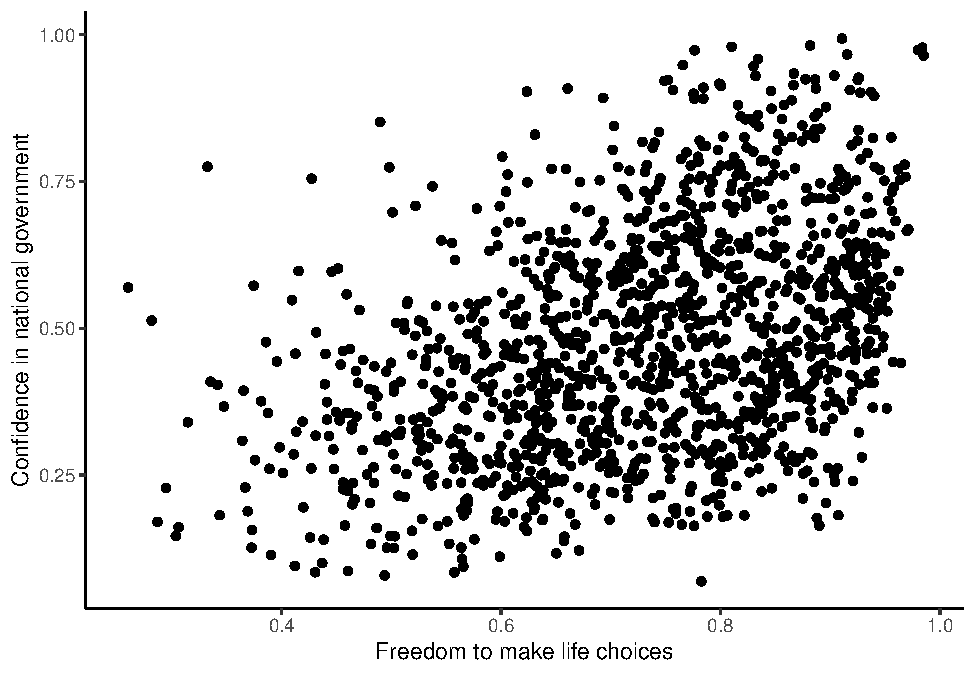
\includegraphics{quantrma_ex_files/figure-latex/unnamed-chunk-39-1.pdf}

Interesting, what happened here? We can see some dots, but the correlation was NA (meaning undefined). This occurred because there are some missing data points in the data. We can remove all the rows with missing data first, then do the correlation. We will do this a couple steps, first creating our own data.frame with only the numbers we want to analyse. We can select the columns we want to keep using \texttt{select}. Then we use \texttt{filter} to remove the rows with NAs.

\begin{verbatim}
## [1] 0.4080963
\end{verbatim}

Now we see the correlation is .408.

Although the scatter plot shows the dots are everywhere, it generally shows that as Freedom to make life choices increases in a country, that countries confidence in their national government also increase. This is a positive correlation. Let's do this again and add the best fit line, so the trend is more clear, we use \texttt{geom\_smooth(method=lm,\ se=FALSE)}. I also change the \texttt{alpha} value of the dots so they blend it bit, and you can see more of them.

\begin{verbatim}
## [1] 0.4080963
\end{verbatim}

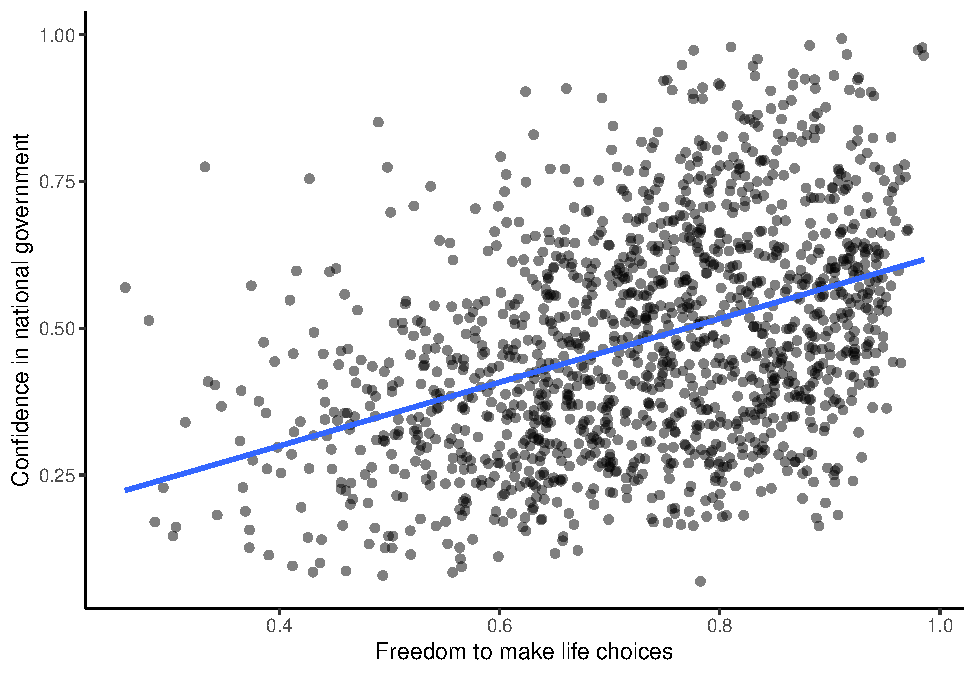
\includegraphics{quantrma_ex_files/figure-latex/unnamed-chunk-41-1.pdf}

\hypertarget{my-question-2}{%
\subsubsection{My Question \#2}\label{my-question-2}}

After all that work, we can now speedily answer more questions. For example, what is the relationship between positive affect in a country and negative affect in a country. I wouldn't be surprised if there was a negative correlation here: when positive feelings generally go up, shouldn't negative feelings generally go down?

To answer this question, we just copy paste the last code block, and change the DVs to be \texttt{Positive\ affect}, and \texttt{Negative\ affect}

\begin{verbatim}
## [1] -0.3841123
\end{verbatim}

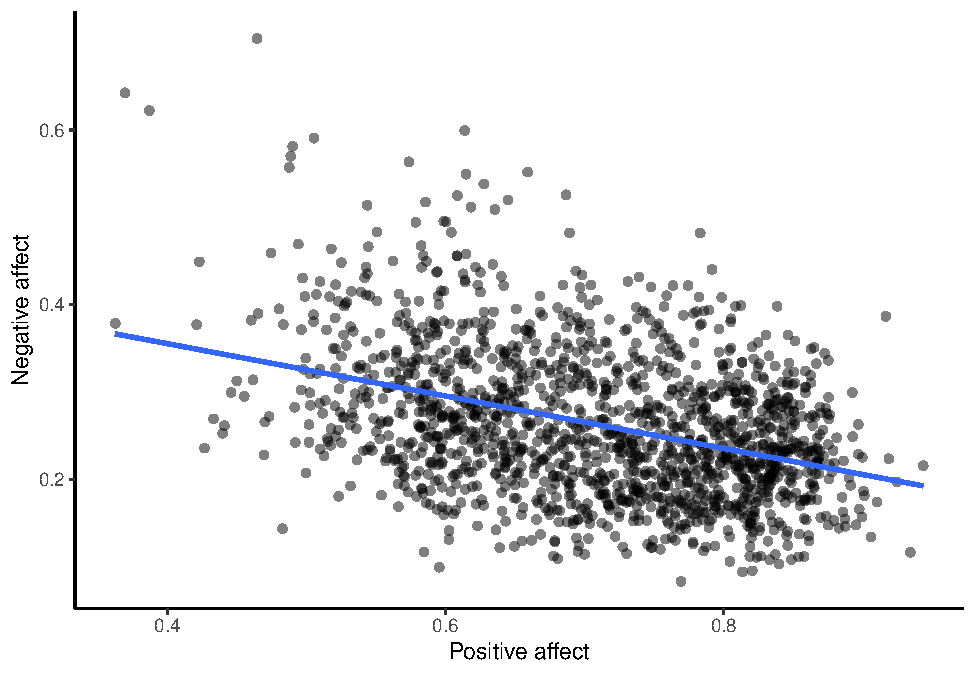
\includegraphics{quantrma_ex_files/figure-latex/unnamed-chunk-42-1.pdf}

Bam, there we have it. As positive affect goes up, negative affect goes down. A negative correlation.

\hypertarget{generalization-exercise-2}{%
\subsection{Generalization Exercise}\label{generalization-exercise-2}}

This generalization exercise will explore the idea that correlations between two measures can arise by chance alone. There are two questions to answer. For each question you will be sampling random numbers from uniform distribution. To conduct the estimate, you will be running a simulation 100 times. The questions are:

\begin{enumerate}
\def\labelenumi{\arabic{enumi}.}
\item
  Estimate the range (minimum and maximum) of correlations (using pearons's r) that could occur by chance between two variables with n=10.
\item
  Estimate the range (minimum and maximum) of correlations (using pearons's r) that could occur bychance between two variables with n = 100.
\end{enumerate}

Use these tips to answer the question.

Tip 1: You can use the \texttt{runif()} function to sample random numbers between a minimum value, and maximum value. The example below sample 10 (n=10) random numbers between the range 0 (min = 0) and 10 (max=10). Everytime you run this code, the 10 values in x will be re-sampled, and will be 10 new random numbers

Tip 2: You can compute the correlation between two sets of random numbers, by first sampling random numbers into each variable, and then running the \texttt{cor()} function.

\begin{verbatim}
## [1] -0.08494266
\end{verbatim}

Running the above code will give different values for the correlation each time, because the numbers in x and y are always randomly different. We might expect that because x and y are chosen randomly that there should be a 0 correlation. However, what we see is that random sampling can produce ``fake'' correlations just by chance alone. We want to estimate the range of correlations that chance can produce.

Tip 3: One way to estimate the range of correlations that chance can produce is to repeat the above code many times. For example, if you ran the above code 100 times, you could save the correlations each time, then look at the smallest and largest correlation. This would be an estimate of the range of correlations that can be produced by chance. How can you repeat the above code many times to solve this problem?

We can do this using a \texttt{for} loop. The code below shows how to repeat everything inside the for loop 100 times. The variable \texttt{i} is an index, that goes from 1 to 100. The \texttt{saved\_value} variable starts out as an empty variable, and then we put a value into it (at index position i, from 1 to 100). In this code, we put the sum of the products of x and y into the \texttt{saved\_value} variable. At the end of the simulation, the \texttt{save\_value} variable contains 100 numbers. The \texttt{min()} and \texttt{max()} functions are used to find the minimum and maximum values for each of the 100 simulations. You should be able to modify this code by replacing \texttt{sum(x*y)} with \texttt{cor(x,y)}. Doing this will allow you to run the simulation 100 times, and find the minimum correlation and maximum correlation that arises by chance. This will be estimate for question 1. To provide an estimate for question 2, you will need to change \texttt{n=10} to \texttt{n=100}.

\begin{verbatim}
## [1] 108.2401
\end{verbatim}

\begin{verbatim}
## [1] 463.0639
\end{verbatim}

\hypertarget{writing-assignment-2}{%
\subsection{Writing assignment}\label{writing-assignment-2}}

Answer the following questions with complete sentences. When you have finished everything. Knit the document and hand in your stuff (you can submit your .RMD file to blackboard if it does not knit.)

\begin{enumerate}
\def\labelenumi{\arabic{enumi}.}
\item
  Imagine a researcher found a positive correlation between two variables, and reported that the r value was +.3. One possibility is that there is a true correlation between these two variables. Discuss one alternative possibility that would also explain the observation of +.3 value between the variables.
\item
  Explain the difference between a correlation of r = .3 and r = .7. What does a larger value of r represent?
\item
  Explain the difference between a correlation of r = .5, and r = -.5.
\end{enumerate}

  \bibliography{QuantRMA\_Ex.bib}

\end{document}
